% Laporan IF4031 Milestone 2 -- dibangkitkan dari docs/report/m2/*.md oleh tools/report/md2tex.py
\documentclass[11pt,a4paper,oneside]{report}
\usepackage{fontspec}
\setmainfont{texgyrepagella}[Extension=.otf,UprightFont=*-regular,BoldFont=*-bold,ItalicFont=*-italic,BoldItalicFont=*-bolditalic]
\setsansfont{texgyreheros}[Extension=.otf,UprightFont=*-regular,BoldFont=*-bold,ItalicFont=*-italic,BoldItalicFont=*-bolditalic,Scale=MatchLowercase]
\setmonofont{lmmono10-regular}[Extension=.otf,BoldFont=lmmonolt10-bold,ItalicFont=lmmono10-italic,BoldItalicFont=lmmonolt10-boldoblique,Scale=MatchLowercase]
\usepackage[indonesian]{babel}
\usepackage[a4paper,margin=2.4cm,headheight=14pt]{geometry}
\usepackage{microtype}
\usepackage{setspace}
\setstretch{1.12}
\usepackage{parskip}
\setlength{\parskip}{0.55em}
\usepackage{xcolor}
\usepackage{booktabs,tabularx,array,longtable,multirow}
\usepackage{enumitem}
\setlist{nosep,leftmargin=1.4em,itemsep=0.2em}
\usepackage{url}
\urlstyle{tt}
\makeatletter
\g@addto@macro\UrlBreaks{\do\_\do\=\do\:\do\,}
\g@addto@macro\UrlBigBreaks{\do\_\do\[\do\]\do\(\do\)}
\makeatother
\Urlmuskip=0mu plus 0.5mu
\emergencystretch=2.5em
\usepackage{listings}
\usepackage{tikz}
\usetikzlibrary{positioning,fit,backgrounds,arrows.meta,shapes.geometric,calc}
\usepackage[most]{tcolorbox}
\usepackage{fancyhdr}
\usepackage{titlesec}
\usepackage{caption}
\usepackage[hidelinks]{hyperref}

% ---- warna
\definecolor{ink}{HTML}{000000}
\definecolor{accent}{HTML}{000000}
\definecolor{accentlight}{HTML}{EBEBEB}
\definecolor{okgreen}{HTML}{000000}
\definecolor{okbg}{HTML}{F5F5F5}
\definecolor{warnorange}{HTML}{000000}
\definecolor{warnbg}{HTML}{F0F0F0}
\definecolor{todored}{HTML}{000000}
\definecolor{gridgray}{HTML}{808080}
\definecolor{codebg}{HTML}{F5F5F5}
\color{ink}

% ---- judul bagian
\titleformat{\chapter}[hang]{\sffamily\bfseries\huge\color{accent}}{\thechapter}{0.6em}{}
\titlespacing*{\chapter}{0pt}{-10pt}{22pt}
\titleformat{\section}{\sffamily\bfseries\Large\color{accent}}{\thesection}{0.6em}{}
\titleformat{\subsection}{\sffamily\bfseries\large\color{ink}}{\thesubsection}{0.6em}{}
\titleformat{\subsubsection}{\sffamily\bfseries\normalsize\color{ink}}{}{0em}{}
\titlespacing*{\section}{0pt}{1.6em}{0.5em}
\titlespacing*{\subsection}{0pt}{1.2em}{0.4em}

% ---- header/footer
\pagestyle{fancy}
\fancyhf{}
\renewcommand{\headrulewidth}{0.3pt}
\fancyhead[L]{\sffamily\footnotesize IF4031 -- Laporan Milestone 2}
\fancyhead[R]{\sffamily\footnotesize ARGUS -- Aggregated Real-time Geohazard Unified System}
\fancyfoot[C]{\sffamily\footnotesize\thepage}

% ---- tampilan kode / log
\lstset{
  basicstyle=\ttfamily\scriptsize,
  backgroundcolor=\color{codebg},
  frame=single, rulecolor=\color{gridgray!50},
  breaklines=true, breakatwhitespace=false,
  columns=fullflexible, keepspaces=true,
  xleftmargin=2pt, xrightmargin=2pt,
  aboveskip=0.6em, belowskip=0.4em,
  upquote=true,
  literate={—}{{\textemdash}}1
}
% \code: tanpa spasi, boleh putus baris di / _ - . ; \cmd: mempertahankan spasi (perintah terminal).
\newcommand{\code}[1]{\path{#1}}
\newcommand{\cmd}[1]{\texttt{\detokenize{#1}}}
\newcommand{\todo}[1]{\textcolor{todored}{\textbf{[#1]}}}

% ---- kotak
\newtcolorbox{ringkas}[1][Ringkasan]{
  enhanced, breakable, colback=accentlight, colframe=accent, boxrule=0.5pt,
  left=6pt,right=6pt,top=4pt,bottom=4pt, fonttitle=\sffamily\bfseries\small, title={#1}}
\newtcolorbox{jawaban}[1][Inti jawaban]{
  enhanced, breakable, colback=okbg, colframe=okgreen, boxrule=0.5pt,
  left=6pt,right=6pt,top=4pt,bottom=4pt, fonttitle=\sffamily\bfseries\small, title={#1}}
\newtcolorbox{catatan}[1][Catatan]{
  enhanced, breakable, colback=warnbg, colframe=warnorange, boxrule=0.5pt,
  left=6pt,right=6pt,top=4pt,bottom=4pt, fonttitle=\sffamily\bfseries\small, title={#1}}

% ---- tabel
\renewcommand{\arraystretch}{1.18}
\newcolumntype{L}[1]{>{\raggedright\arraybackslash}p{#1}}
\newcolumntype{Y}{>{\raggedright\arraybackslash}X}
\captionsetup{font={small,sf},labelfont=bf,skip=4pt}
\newcommand{\lulus}{\textcolor{okgreen}{\textbf{Lulus}}}
\newcommand{\sebagian}{\textcolor{warnorange}{\textbf{Sebagian}}}
\newcommand{\belum}{\textcolor{todored}{\textbf{Belum}}}

\usepackage{graphicx}
\usepackage{float}
\usepackage{pdfpages}
\begin{document}
\begin{titlepage}
\thispagestyle{empty}
\sffamily
\vspace*{1.2cm}
{\color{accent}\rule{\textwidth}{1.6pt}}\\[1.2em]
{\Large IF4031 Arsitektur Aplikasi Terdistribusi}\\[0.4em]
{\large Tugas Besar -- Milestone 2: Sistem Terdistribusi Skalabel}\\[2.2em]
{\fontsize{40}{44}\selectfont\bfseries\color{accent} ARGUS}\\[0.5em]
{\Large\bfseries Aggregated Real-time Geohazard Unified System}\\[0.8em]
{\large Gateway kebencanaan BNPB di atas Kubernetes}\\[1.2em]
{\color{accent}\rule{\textwidth}{0.6pt}}

\vspace{2.2cm}
\begin{tabular}{@{}L{3.6cm}L{10cm}@{}}
\textbf{Nama kelompok} & OrangSuksesAamiin\\[0.8em]
\textbf{Anggota} & 13523128 - Andi Farhan Hidayat\\
 & 13523164 - Muhammad Rizain Firdaus\\
 & 13523152 - Muhammad Kinan Arkansyaddad\\[0.8em]
\textbf{Mata kuliah} & IF4031 Arsitektur Aplikasi Terdistribusi\\
\textbf{Institusi} & Institut Teknologi Bandung\\
\textbf{Semester} & 7, 2026/2027
\end{tabular}

\vfill
{\small\color{gridgray}Berkas ini dikumpulkan sebagai \texttt{IF4031\_M2\_OrangSuksesAamiin.pdf}.}
\end{titlepage}
\pagenumbering{roman}
\tableofcontents
\clearpage
\pagenumbering{arabic}
\chapter{Bagian Umum}

\section{Tabel kontribusi}

{\small
\begin{longtable}{@{}>{\raggedright\arraybackslash}p{0.145\linewidth}>{\raggedright\arraybackslash}p{0.273\linewidth}>{\raggedright\arraybackslash}p{0.283\linewidth}>{\raggedright\arraybackslash}p{0.221\linewidth}@{}}
\toprule
\textbf{Anggota} & \textbf{Perancangan} & \textbf{Implementasi} & \textbf{Penulisan laporan} \\
\midrule
\endhead
13523128 -- Andi Farhan Hidayat (Orang 1) & Platform Kubernetes, satu penulis ber-fencing, kebijakan skema dan DLQ, integrasi akhir & Manifest k8s dan satu perintah deploy, cluster VirtualBox, leader election + fencing (P2), DLQ dan mode skema tidak kompatibel (P3 kriteria 1--5), Audit \texttt{unprocessed}, integrasi M2: storage sharded di 2 node, \texttt{balance-\allowbreak{}shard}, metrik penempatan dan feed, demo P1/P5 game day, gladi penuh di k3s & Bagian umum, P2, P3 (1--5), penyuntingan P1 dan P4, penyusunan PDF \\
13523164 -- Muhammad Rizain Firdaus (Orang 2) & Observabilitas, jalur laporan Tim Lapangan, ketahanan Sensor Pantai, admisi per peran & \texttt{pkg/\allowbreak{}obs} (metrik Prometheus, trace W3C), Grafana/Prometheus/Jaeger, \texttt{POST /\allowbreak{}v1/\allowbreak{}field-\allowbreak{}reports} + pemroses exactly-once (P3 kriteria 6), Sensor Pantai (P5), dashboard analitik (P1 kriteria 7), load test k6, HPA & Observabilitas, P3 kriteria 6, P5, P1 kriteria 7, konfigurasi load test \\
13523152 -- Muhammad Kinan Arkansyaddad (Orang 3) & Canonical Store terdistribusi (Patroni per shard), Audit API, pemrosesan aliran satelit & Adapter \texttt{sharded}, migrasi store tunggal $\rightarrow$ sharded, Audit \texttt{events}/\texttt{checksum}/\texttt{location}, consumer SSE Feed Satelit dan pengelompokan kebakaran (P4), cluster QEMU 3 node & Draf P1 dan P4 \\
\bottomrule
\end{longtable}
}

\section{Deskripsi umum sistem}

ARGUS adalah gateway kebencanaan BNPB yang menyatukan beberapa sumber ke satu format \textbf{HazardEvent}:

\begin{itemize}
\item BMKG (gempa, peringatan tsunami)
\item PVMBG (gunung api)
\item Feed Satelit (titik panas $\rightarrow$ kebakaran hutan)
\item Sensor Pantai (pengamatan pesisir).
\end{itemize}

Setiap HazardEvent disimpan di \textbf{Canonical Store}, yang hanya dimiliki Aggregator. Event diterbitkan ke Kafka lewat outbox, lalu disajikan kepada Media, Tim Lapangan, dan BNPB Pusat sesuai hak masing-masing.


M2 menjalankan sistem yang sama di Kubernetes dengan dua node berkernel terpisah. Perubahannya:

\begin{itemize}
\item Canonical Store dibagi menjadi 3 shard yang direplikasi ke node lain.
\item Aggregator berjalan $\ge$ 3 instance di belakang satu Service, dan hanya satu leader ber-fencing yang mengambil data.
\item Pesan yang gagal disimpan utuh di dead-letter store.
\item Feed Satelit dibaca sebagai aliran SSE dengan offset.
\item Sensor Pantai diisolasi dengan bulkhead dan circuit breaker.
\item Tim Lapangan dapat mengirim laporan yang dijamin diproses tepat sekali.
\end{itemize}

\section{Diagram arsitektur}

\begin{figure}[H]\centering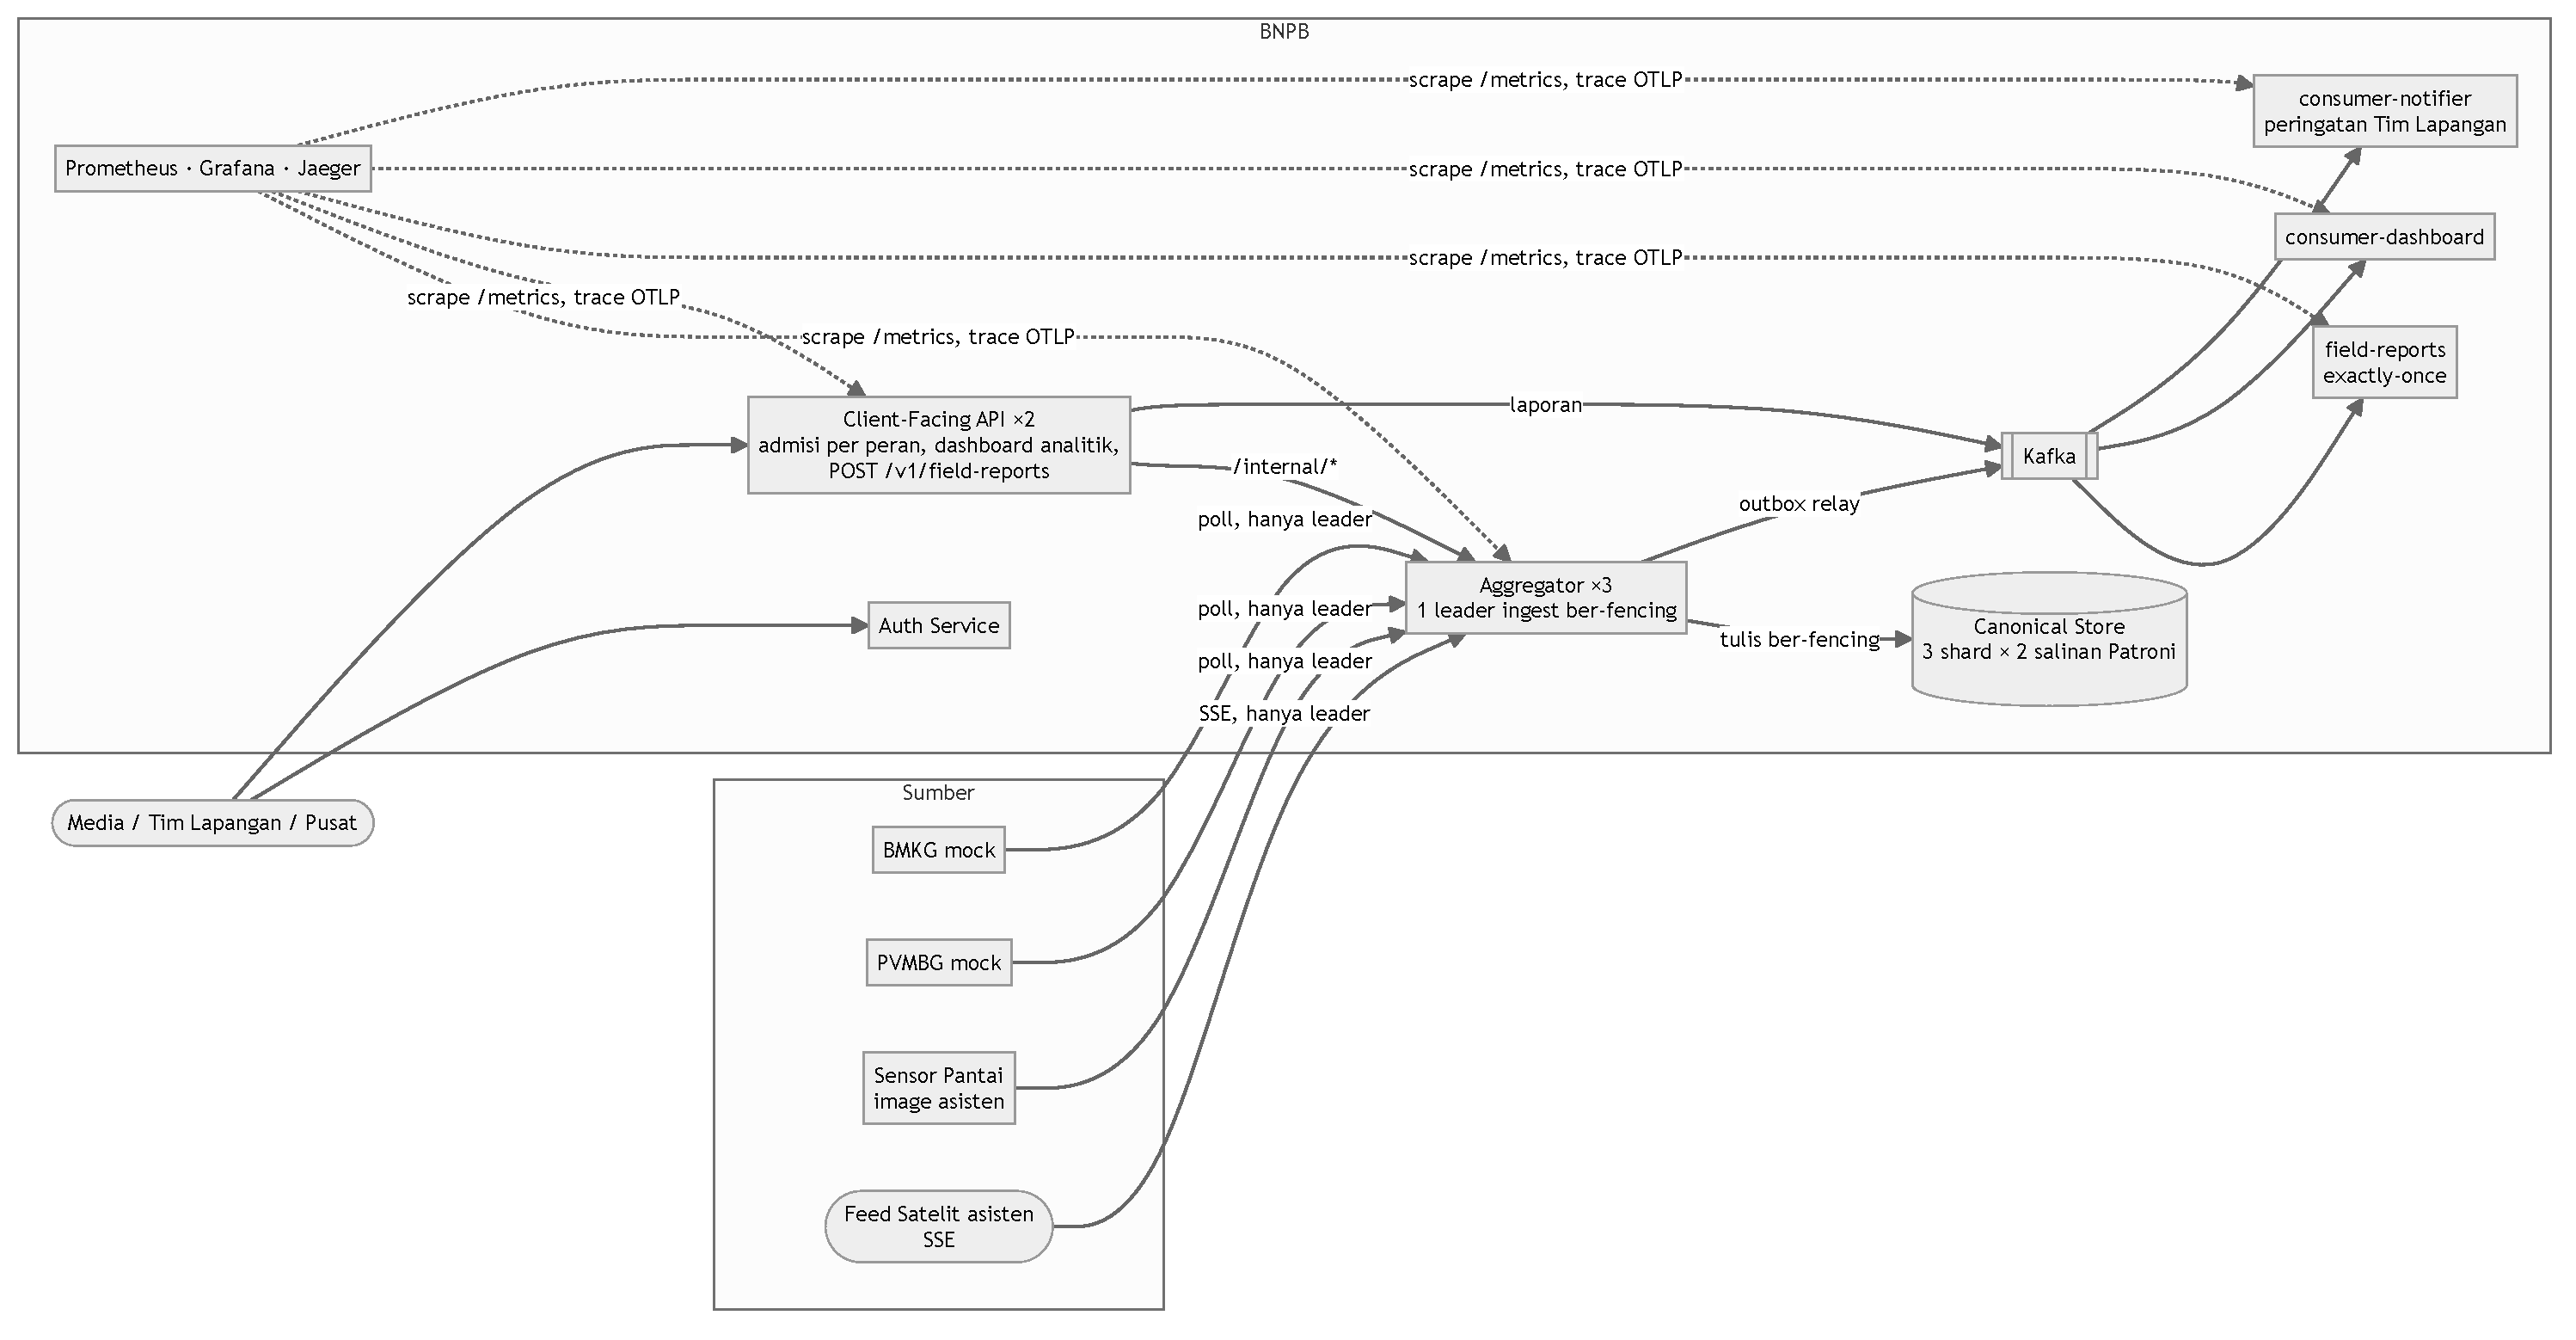
\includegraphics[width=\linewidth,height=0.82\textheight,keepaspectratio]{fig/m1.pdf}\end{figure}

\section{Daftar teknologi terpilih}

{\small
\begin{longtable}{@{}>{\raggedright\arraybackslash}p{0.119\linewidth}>{\raggedright\arraybackslash}p{0.365\linewidth}>{\raggedright\arraybackslash}p{0.450\linewidth}@{}}
\toprule
\textbf{Bagian} & \textbf{Teknologi} & \textbf{Alasan singkat} \\
\midrule
\endhead
Bahasa service & Go 1.25 (\texttt{net/\allowbreak{}http}, \texttt{log/\allowbreak{}slog}) & Biner statis kecil, cocok dengan limit memori Lampiran B \\
Orkestrasi & k3s v1.37 di 2 VM VirtualBox (Ubuntu 24.04) & Ringan, NetworkPolicy, Lease, local-path PV bawaan \\
Canonical Store & PostgreSQL 16 + JSONB, Patroni 4.1 per shard (DCS = API Kubernetes) & Transaksi untuk outbox + fence, replikasi sinkron dan failover tanpa etcd tambahan \\
Broker & Kafka (KRaft), transaksi untuk field reports & Log berurutan, consumer group, exactly-once producer \\
Koordinasi leader & Lease \texttt{coordination.\allowbreak{}k8s.\allowbreak{}io} + fencing token di store & Jam kebenaran = API server, bukan jam node \\
Observabilitas & Prometheus, Grafana, Jaeger (OTLP), log JSON ber-\texttt{cid} & Satu dashboard, trace lintas service \\
Load test & k6 (di host, di luar pod) & 10.000 VU, skenario ber-peran \\
Uji ketahanan & Tester Agent asisten (image dipin digest) & Ketentuan M2 \\
\bottomrule
\end{longtable}
}

\section{Asumsi}

\begin{itemize}
\item Semua node berada dalam satu jaringan dengan latensi rendah (VirtualBox NAT Network). Bonus host fisik berbeda tidak diambil.
\item Data \texttt{role=\allowbreak{}store} cukup disimpan di disk lokal node (local-path PV), tidak ada backup ke luar cluster.
\item Katalog gempa dari asisten belum diterima saat bukti diambil. P1 memakai katalog sintetis yang meniru kemiringan wilayah (\texttt{tools/\allowbreak{}catalog/\allowbreak{}catalog.\allowbreak{}py}). Katalog asli dapat dimuat tanpa perubahan kode.
\item \texttt{AUDIT\_\allowbreak{}TOKEN}, kunci skenario ujian, dan token sesi ujian baru diberikan setelah tenggat. Bukti di laporan ini memakai token pengembangan dan skenario practice, hasil ujian ditunjukkan di video.
\end{itemize}

\section{Petunjuk menjalankan}

README §M2 berisi langkah lengkap dari kondisi awal, daftar variabel konfigurasi, dan cara memicu setiap skenario. Ringkasannya ada di Lampiran A. Intinya: \texttt{bash scripts/\allowbreak{}k8s/\allowbreak{}vbox-\allowbreak{}cluster.\allowbreak{}sh up}, \texttt{cp .\allowbreak{}env.\allowbreak{}example .\allowbreak{}env}, lalu \texttt{make k8s-\allowbreak{}up}.


\section{Diagram deployment}

\begin{figure}[H]\centering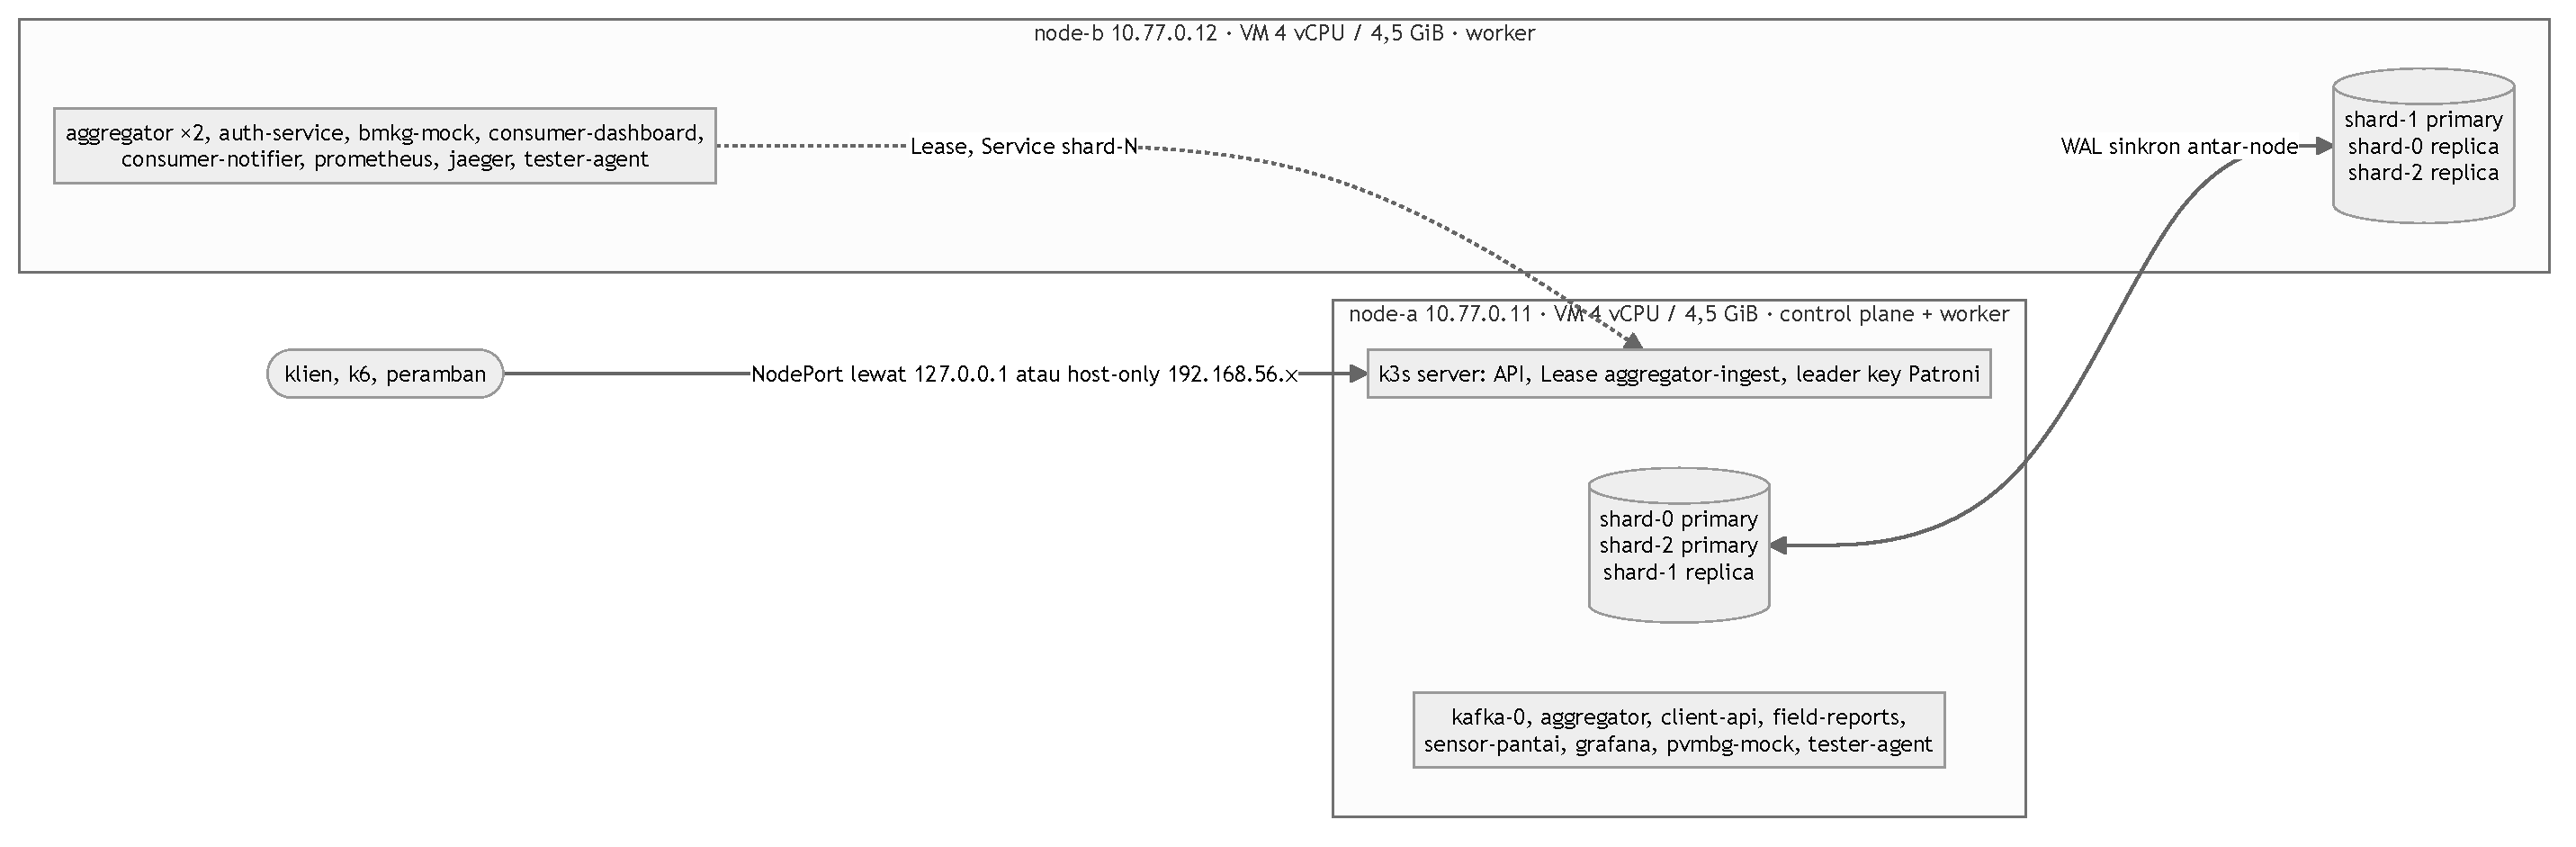
\includegraphics[width=\linewidth,height=0.82\textheight,keepaspectratio]{fig/m2.pdf}\end{figure}

Penempatan stateless (aggregator, client-api, consumer, observabilitas) ditentukan scheduler dan dapat berbeda di setiap deploy. \texttt{make k8s-\allowbreak{}status} dan \texttt{kubectl get pods -\allowbreak{}o wide -\allowbreak{}L role,\allowbreak{}db-\allowbreak{}role} menunjukkan keadaan terkini. Yang \textbf{dijamin} manifest:

\begin{itemize}
\item Dua salinan setiap shard berada di node berbeda (pod anti-affinity wajib).
\item Primary pilihan tiap shard dirotasi di node (ConfigMap \texttt{shard-\allowbreak{}placement}, dikembalikan oleh \texttt{balance-\allowbreak{}shard}).
\item Aggregator tersebar dengan selisih $\le$ 1 per node (\texttt{topology\allowbreak{}Spread\allowbreak{}Constraints}).
\item Data \texttt{role=\allowbreak{}store} dan \texttt{role=\allowbreak{}broker} disimpan di disk node (local-path PV).
\item Tester Agent berjalan satu per node.
\end{itemize}

Jalur data antar-node: replikasi WAL Patroni (5432) antar anggota shard, Service $\rightarrow$ primary shard, kube-proxy untuk Service lain, dan Lease/Endpoints lewat API server di node-a. NetworkPolicy hanya mengizinkan Aggregator (dan Job migrasi) membuka koneksi ke store, dan hanya klien Kafka berlabel yang boleh ke broker.


\section{Perubahan dari M1}

{\small
\begin{longtable}{@{}>{\raggedright\arraybackslash}p{0.284\linewidth}>{\raggedright\arraybackslash}p{0.398\linewidth}>{\raggedright\arraybackslash}p{0.252\linewidth}@{}}
\toprule
\textbf{Keputusan M1} & \textbf{M2} & \textbf{Alasan} \\
\midrule
\endhead
\texttt{docker compose}, satu host & \textbf{Diubah}: Kubernetes (k3s), manifest \texttt{deploy/\allowbreak{}}, satu perintah \texttt{make k8s-\allowbreak{}up}, compose tetap untuk pengembangan & Ketentuan M2, banyak node, rolling update, self-healing \\
Satu PostgreSQL sebagai Canonical Store & \textbf{Diubah}: 3 shard Patroni $\times$ 2 salinan di node berbeda, hash \texttt{hazard\_\allowbreak{}id}, migrasi online \texttt{MIGRATE\_\allowbreak{}CANONICAL=\allowbreak{}1} & P1: tidak muat di satu tempat, harus tahan kehilangan node \\
Isolasi storage lewat jaringan Docker internal & \textbf{Diubah}: NetworkPolicy + Secret per komponen & Ditegakkan platform di cluster \\
Satu Aggregator yang polling & \textbf{Diubah}: $\ge$ 3 instance, satu leader (Lease) yang ingest, semua melayani baca, fencing token di setiap shard & P2: tanpa ini tiap kejadian diambil tiga kali \\
Polling untuk semua sumber & \textbf{Dipertahankan} untuk BMKG/PVMBG/Sensor Pantai, \textbf{tidak dipakai} untuk Feed Satelit (SSE + offset) & P4 §2 \\
Status sumber di memori Aggregator & \textbf{Diubah}: disimpan leader di store, dibaca semua instance & Freshness yang sama di setiap instance \\
Karantina di memori & \textbf{Diganti}: dead-letter store persisten (raw bytes, retrying/parked), hanya untuk Internal Ops & P3 \\
Parser JSON standar & \textbf{Diganti}: pemecah array streaming per elemen dengan batas ukuran/kedalaman & P3: satu pesan rusak tidak menjatuhkan batch \\
Kebijakan skema additive-only, perubahan tak didukung dikarantina & \textbf{Dipertahankan}, ditambah aturan penyesuaian deklaratif (\texttt{rename}, \texttt{coerce}) & Tetap tidak menebak \\
Outbox transaksional + relay, Kafka at-least-once & \textbf{Dipertahankan}, outbox ikut shard hazard-nya, relay hanya di leader & Audit siapa menulis apa per term \\
Client API hanya baca & \textbf{Diubah}: \texttt{POST /\allowbreak{}v1/\allowbreak{}field-\allowbreak{}reports} (202 setelah Kafka mengonfirmasi), admisi per peran & P3 kriteria 6, P5 kriteria 5 \\
Log JSON ber-\texttt{cid} & \textbf{Dipertahankan}, ditambah metrik Prometheus dan trace W3C & Observabilitas M2 \\
Admin mock wajib \texttt{X-\allowbreak{}Admin-\allowbreak{}Token} & \textbf{Diubah di k8s}: boleh tanpa token (\texttt{*\_\allowbreak{}ADMIN\_\allowbreak{}OPEN}), Service mock hanya ClusterIP & Tester Agent memanggil \texttt{/\allowbreak{}admin/\allowbreak{}*} tanpa kredensial \\
\bottomrule
\end{longtable}
}

\section{Deklarasi topologi}

{\small
\begin{longtable}{@{}>{\raggedright\arraybackslash}p{0.104\linewidth}>{\raggedright\arraybackslash}p{0.104\linewidth}>{\raggedright\arraybackslash}p{0.104\linewidth}>{\raggedright\arraybackslash}p{0.104\linewidth}>{\raggedright\arraybackslash}p{0.135\linewidth}>{\raggedright\arraybackslash}p{0.154\linewidth}>{\raggedright\arraybackslash}p{0.181\linewidth}@{}}
\toprule
\textbf{Node} & \textbf{Peran} & \textbf{Jenis} & \textbf{vCPU / RAM} & \textbf{OS / kernel} & \textbf{Host fisik} & \textbf{CPU / RAM host} \\
\midrule
\endhead
node-a (10.77.0.11) & control plane + worker & VM VirtualBox 7.1.4 & 4 / 4,5 GiB, disk 10 GB & Ubuntu 24.04.5, 6.8.0-147, k3s v1.37.2 & Laptop Acer Nitro AN515-58, Windows 11 Home & Intel Core i5-12500H (12 core / 16 thread) / 24 GB \\
node-b (10.77.0.12) & worker & VM VirtualBox 7.1.4 & 4 / 4,5 GiB, disk 10 GB & idem & laptop yang sama & sama \\
\bottomrule
\end{longtable}
}

Kedua node berkernel terpisah (boot id berbeda, \texttt{docs/\allowbreak{}evidence/\allowbreak{}m2/\allowbreak{}topology.\allowbreak{}log}). Skenario mematikan node hanya dikenakan pada node-b (worker non-control-plane).


\section{Observabilitas}

Setiap service BNPB memakai \texttt{pkg/\allowbreak{}obs}, sehingga ketiga syarat observabilitas berlaku seragam tanpa kode per service:


\begin{enumerate}
\item \textbf{Metrik dalam satu dashboard.} Setiap service melayani \texttt{GET /\allowbreak{}metrics}: jumlah, latensi (histogram) dan status per route, panggilan keluar per tujuan, serta metrik domain. Metrik domain mencakup status sumber dan breaker, leader dan term, outbox, DLQ, Sensor Pantai, admisi per peran, laporan lapangan, consumer, penempatan unit penyimpanan per node, beban tulis per shard, serta lag dan latensi Feed Satelit. Prometheus menemukan setiap pod sendiri, dan Grafana menampilkan satu dashboard ``Argus / Observabilitas'' (\texttt{:30030}).
\item \textbf{Trace satu permintaan lintas service.} Konteks W3C \texttt{traceparent} dibawa lewat HTTP dan header Kafka, lalu diekspor ke Jaeger (\texttt{:30686}). Durasi tiap langkah terlihat, misalnya client-api $\rightarrow$ aggregator $\rightarrow$ store, client-api $\rightarrow$ Kafka $\rightarrow$ field-reports, dan poll $\rightarrow$ upstream $\rightarrow$ store $\rightarrow$ outbox $\rightarrow$ Kafka $\rightarrow$ consumer.
\item \textbf{Log terstruktur ber-correlation ID.} Format log M1 dipertahankan, dengan tambahan \texttt{trace\_\allowbreak{}id}.
\end{enumerate}

\texttt{pkg/\allowbreak{}obs} tanpa dependensi pihak ketiga: registry Prometheus dan exporter OTLP/HTTP JSON ditulis sendiri, agar tidak ada SDK yang menambah memori pod (Lampiran B). Komponen observabilitas di-deploy dengan \texttt{role=\allowbreak{}other} dan 128/256 Mi. Demo: \texttt{make demo-\allowbreak{}m2-\allowbreak{}observability}.


\textbf{Bukti.} Demo otomatis \texttt{make demo-\allowbreak{}m2-\allowbreak{}observability} lulus di cluster pengembangan kind (\texttt{docs/\allowbreak{}evidence/\allowbreak{}m2/\allowbreak{}observability-\allowbreak{}kind.\allowbreak{}log}): metrik setiap service ter-scrape, satu trace lintas service dengan durasi tiap langkah, serta \texttt{cid} dan \texttt{trace\_\allowbreak{}id} di log. Di cluster demo k3s, Grafana (\texttt{:30030}, NIC host-only \texttt{192.\allowbreak{}168.\allowbreak{}56.\allowbreak{}11}), Prometheus, dan Jaeger berjalan dan menampilkan baris dashboard baru untuk penempatan storage (P1) dan ketertinggalan Feed Satelit (P4). Demo otomatisnya tidak diulang di k3s karena waktu. Tampilan langsung ditunjukkan di video.


\chapter{Problem 1 --- Yang Pulang Membawa Laptopnya}

\section{Identifikasi masalah (butir ``Di laporan'' 1)}

{\small
\begin{longtable}{@{}>{\raggedright\arraybackslash}p{0.405\linewidth}>{\raggedright\arraybackslash}p{0.541\linewidth}@{}}
\toprule
\textbf{Persoalan} & \textbf{Nama dan konsep dalam literatur} \\
\midrule
\endhead
Data tidak muat di satu penyimpanan dan harus dibagi & \textbf{Partitioning / sharding} (Kleppmann, \emph{DDIA} bab 6): setiap record punya tepat satu partisi pemilik. \\
Gempa terkonsentrasi di satu jalur sehingga satu mesin bekerja keras & \textbf{Data skew} dan \textbf{hot spot / hot partition}. Partisi menurut kunci yang berkorelasi dengan wilayah atau waktu menumpuk beban di satu partisi. \\
Laptop pulang membawa sebagian catatan & \textbf{Replication} untuk \emph{durability} dan \emph{availability}: \emph{single-leader (primary--backup) replication} dengan \emph{synchronous standby}, \textbf{failover}, dan bahaya \textbf{split-brain}. \\
Laptop baru harus masuk tanpa mematikan sistem & \textbf{Rebalancing}: memindahkan salinan dan peran primary ke node baru secara online (\emph{re-replication}, \emph{planned switchover}). \\
Membaca lintas lokasi selama sebagian unit hilang & \textbf{Scatter--gather} dengan batas waktu per unit; \textbf{degraded / partial results} (\emph{harvest vs yield}, Fox \& Brewer 1999); trade-off konsistensi--ketersediaan (\textbf{CAP/PACELC}). \\
\bottomrule
\end{longtable}
}

\section{Mekanisme yang dipilih (butir ``Di laporan'' 2)}

\begin{figure}[H]\centering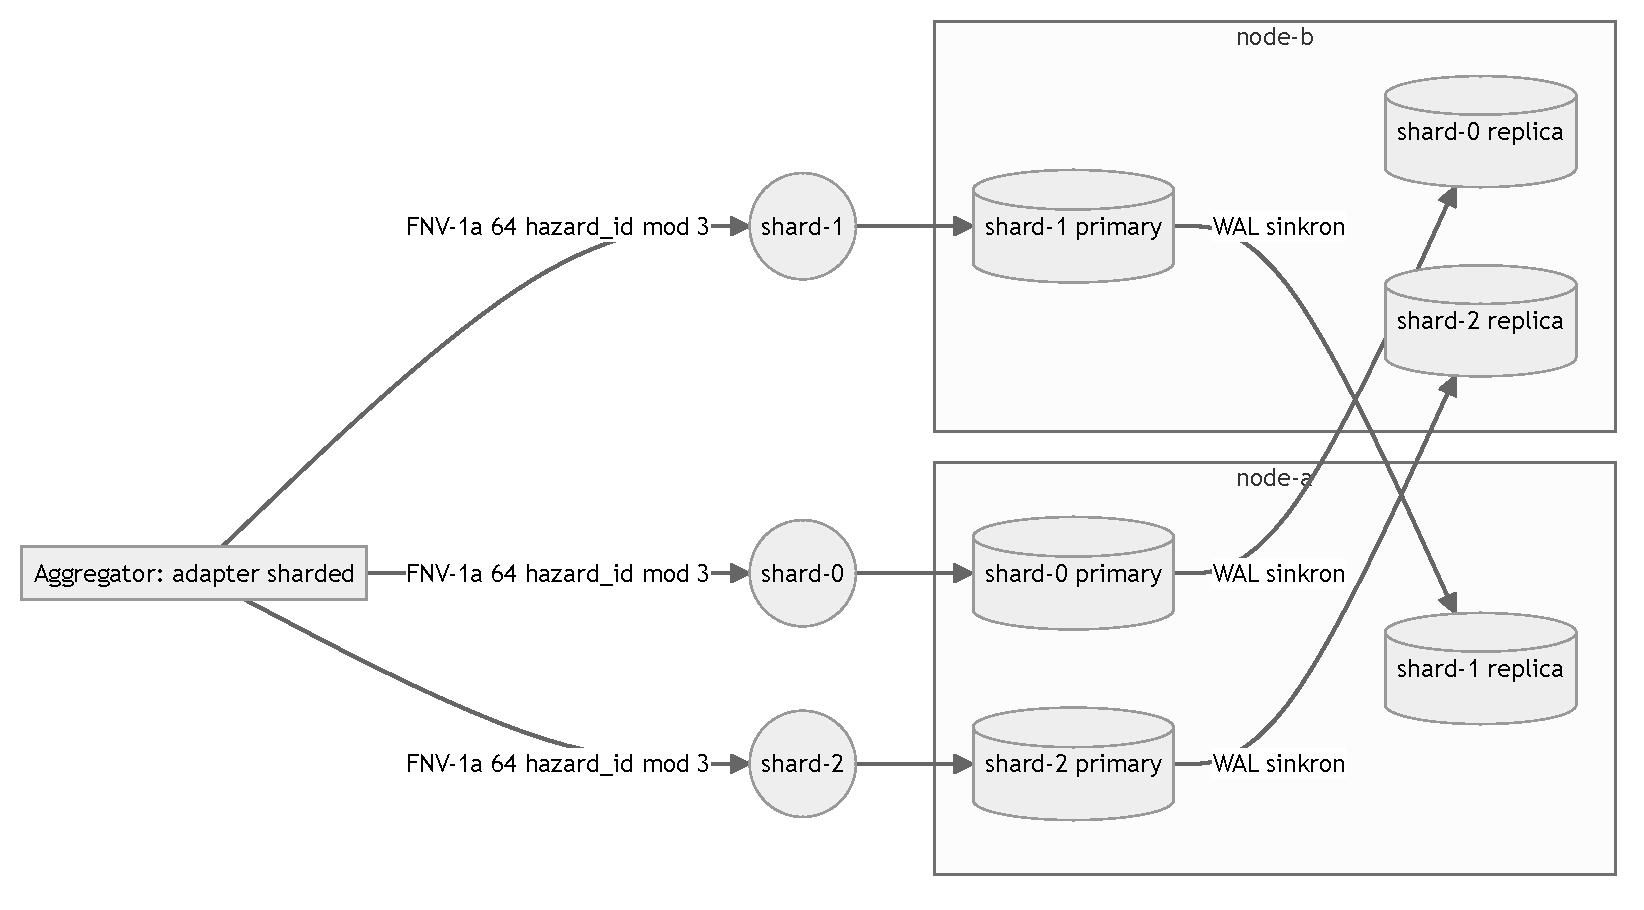
\includegraphics[width=\linewidth,height=0.82\textheight,keepaspectratio]{fig/m3.pdf}\end{figure}

\textbf{Unit penyimpanan.} Canonical Store dibagi menjadi tiga shard logis. Setiap shard adalah satu grup Patroni dengan dua anggota PostgreSQL 16. Kedua anggota berada di node berbeda karena \emph{pod anti-affinity} wajib. Datanya berada di disk node lewat PV \texttt{local-\allowbreak{}path}. Setiap anggota berlabel \texttt{role=\allowbreak{}store}, dengan requests 512Mi dan limits 1Gi (Lampiran B).


\textbf{Di mana sebuah data disimpan.} Aggregator, satu-satunya pemilik store, menghitung \texttt{FNV-\allowbreak{}1a 64(hazard\_\allowbreak{}id) mod 3}. Baris outbox ikut shard hazard-nya dan ditulis dalam transaksi yang sama. Metadata bersama (cursor polling, status sumber, DLQ, checkpoint satelit) berada di shard-0. Shard logis sebuah hazard \textbf{tidak pernah berubah} ketika node datang dan pergi. Yang berpindah hanyalah lokasi fisik salinan dan peran primary. Akibatnya, rebalancing tidak menyalin ulang data antar-shard. Cara ini berbeda dari \emph{consistent hashing} atas node, yang memindahkan kunci saat keanggotaan berubah.


\textbf{Siapa primary.} Patroni menyimpan \emph{leader key} tiap shard di API Kubernetes. Ini sumber kebenaran yang sama dengan lease leader Aggregator pada P2, sehingga keputusan primary tidak bergantung pada jam node. Commit menunggu WAL tersimpan di standby (\texttt{synchronous\_\allowbreak{}mode: true}). Bila primary hilang, standby sinkron yang dipromosikan; salinan usang tidak pernah dipromosikan. Bila standby yang hilang, primary tetap menerima tulis dengan satu salinan (mode sinkron non-strict). Pilihan ini menukar perlindungan terhadap kehilangan \textbf{kedua} selama perbaikan dengan ketersediaan tulis.


\textbf{Sebaran beban tulis.} ConfigMap \texttt{shard-\allowbreak{}placement} menetapkan node pilihan primary tiap shard, dirotasi di node penyimpanan (2 node: shard-0 $\rightarrow$ node-a, shard-1 $\rightarrow$ node-b, shard-2 $\rightarrow$ node-a). \texttt{balance-\allowbreak{}shard} berjalan di setiap anggota dan hanya berbicara dengan API Patroni lokal. Bila leader tidak di node pilihannya, dan anggota di node pilihan sudah \texttt{sync\_\allowbreak{}standby}, \emph{streaming}, lag 0, serta stabil 60 s, leader meminta \textbf{switchover terencana}. Tidak ada data hilang karena kandidatnya sinkron. Ada jeda 300 s antar-switchover untuk mencegah \emph{flapping}. Saat cluster dideploy, ketiga primary mula-mula terpilih di node-b. Satu menit kemudian \texttt{balance-\allowbreak{}shard} memindahkan primary shard-0 dan shard-2 ke node-a tanpa intervensi (log: \texttt{"switchover requested" \ldots{} "Successfully switched over to \textbackslash{}"shard-\allowbreak{}0-\allowbreak{}1\textbackslash{}""}).


\textbf{Ketika node datang dan pergi.}

\begin{itemize}
\item \textbf{Node hilang:} anggota di node lain menjadi primary (failover Patroni). Pembacaan dan tulisan pindah ke sana.
\item \textbf{Node kembali kosong / node baru:} anggota yang PV-nya kosong dibangun ulang otomatis oleh Patroni (\texttt{basebackup} dari primary, lalu \emph{streaming}). Setelah sinkron, \texttt{balance-\allowbreak{}shard} mengembalikan primary ke node pilihan, sehingga node itu ikut menanggung tulisan. Untuk node pengganti bernama lain, \texttt{scripts/\allowbreak{}k8s/\allowbreak{}restore-\allowbreak{}shard.\allowbreak{}sh} memindahkan klaim PV ke node baru.
\item \textbf{Fencing P2 tetap berlaku di setiap shard.} \texttt{RaiseFence} menaikkan term di semua shard, dan setiap tulisan memeriksa fence di transaksinya sendiri.
\end{itemize}

\section{Alternatif dan konsekuensinya pada kriteria 2 (butir ``Di laporan'' 3)}

Ketiga strategi diukur offline pada input yang \textbf{sama} dengan yang dimuat ke cluster: katalog 5.000 gempa dengan kemiringan alami (Sumatera Barat terbanyak) ditambah lonjakan 1.500 gempa di Sumatera Barat. Penempatannya dihitung oleh \texttt{tools/\allowbreak{}catalog/\allowbreak{}catalog.\allowbreak{}py distribution} (\texttt{docs/\allowbreak{}evidence/\allowbreak{}m2/\allowbreak{}p1-\allowbreak{}load-\allowbreak{}latest.\allowbreak{}log} §5).


{\small
\begin{longtable}{@{}>{\raggedright\arraybackslash}p{0.281\linewidth}>{\raggedright\arraybackslash}p{0.191\linewidth}>{\raggedright\arraybackslash}p{0.106\linewidth}>{\raggedright\arraybackslash}p{0.225\linewidth}>{\raggedright\arraybackslash}p{0.106\linewidth}@{}}
\toprule
\textbf{Strategi (3 shard)} & \textbf{Seluruh data: baris per shard} & \textbf{max/mean} & \textbf{Tulisan 24 jam terakhir (lonjakan)} & \textbf{max/mean} \\
\midrule
\endhead
**Hash \texttt{hazard\_\allowbreak{}id} (dipilih)** & 2151 / 2178 / 2171 & \textbf{1,01} & 491 / 509 / 500 & \textbf{1,02} \\
Range per \texttt{area\_\allowbreak{}name} & 1897 / 1298 / 3305 & 1,53 & 0 / 0 / 1500 & 3,00 \\
Range per \texttt{occurred\_\allowbreak{}at} (potongan kuantil) & 2166 / 2167 / 2167 & 1,00 & 0 / 0 / 1500 & 3,00 \\
\bottomrule
\end{longtable}
}

\begin{itemize}
\item \textbf{Range per wilayah:} query per wilayah murah (satu shard), tetapi wilayah teraktif menjadi \emph{hot partition} permanen. Seluruh lonjakan Sumatera Barat jatuh ke satu shard.
\item \textbf{Range per waktu:} seimbang untuk data historis dan \emph{range scan} waktu efisien, tetapi \textbf{semua tulisan baru} selalu menuju partisi terbaru (\emph{write hotspot}).
\item \textbf{Hash (dipilih):} tulisan tersebar rata, termasuk saat lonjakan. Konsekuensinya, setiap query lintas wilayah atau waktu harus \emph{scatter--gather} ke semua shard lalu di-\emph{merge}, dan locality per wilayah hilang.
\end{itemize}

\textbf{Sebaran per node} mengikuti letak primary. Dengan 3 shard di 2 node, node-a memegang 2 primary, sehingga beban tulis terukur 71 \% node-a / 29 \% node-b, baik saat katalog dimuat (+4.099 / +1.700 tulisan) maupun saat lonjakan (+1.244 / +519). Ketidakseimbangan ini disebabkan jumlah shard yang tidak habis dibagi jumlah node, bukan oleh kemiringan data. Dengan 3 node, atau 4 shard di 2 node, pembagiannya rata.


\section{Jaminan konsistensi per endpoint (butir ``Di laporan'' 4)}

{\small
\begin{longtable}{@{}>{\raggedright\arraybackslash}p{0.174\linewidth}>{\raggedright\arraybackslash}p{0.254\linewidth}>{\raggedright\arraybackslash}p{0.254\linewidth}>{\raggedright\arraybackslash}p{0.239\linewidth}@{}}
\toprule
\textbf{Endpoint} & \textbf{Kondisi normal} & \textbf{Selama node hilang} & \textbf{Alasan} \\
\midrule
\endhead
Tulis (ingest, satu leader) & Linearizable per hazard: versi + fence dalam satu transaksi di primary, durable di 2 node sebelum ack & Tetap linearizable per hazard setelah failover; ack hanya durable di 1 node sampai replica kembali & Primary tunggal per shard (leader key di API Kubernetes), standby sinkron, fence term \\
\texttt{GET /\allowbreak{}internal/\allowbreak{}hazards}, \texttt{/\allowbreak{}v1/\allowbreak{}hazards} (50 terbaru, pagination) & Urutan global \texttt{(occurred\_\allowbreak{}at,\allowbreak{} hazard\_\allowbreak{}id)} menurun yang benar; keyset cursor stabil & Shard yang tidak menjawab dalam 1,2 s dilewati: jawaban \textbf{partial} dengan \texttt{partial: true} + \texttt{unavailable\_\allowbreak{}units} (bukan 500, bukan menggantung) & Scatter--gather ber-deadline; \emph{harvest} dikorbankan demi \emph{yield} \\
\texttt{GET /\allowbreak{}internal/\allowbreak{}hazards/\allowbreak{}\{id\}} & Read-your-writes dari primary pemilik & 503 bila shard pemilik tidak terjangkau; 404 hanya bila ketiadaan dapat dipastikan & Ketiadaan tidak boleh ditebak \\
\texttt{GET /\allowbreak{}internal/\allowbreak{}audit/\allowbreak{}events} & Urutan menaik \texttt{(ingested\_\allowbreak{}at,\allowbreak{} hazard\_\allowbreak{}id)}, cursor opaque & \texttt{partial: true} dengan nama unit; cursor yang sama dipakai ulang setelah pulih & Sama dengan di atas \\
\texttt{GET /\allowbreak{}internal/\allowbreak{}audit/\allowbreak{}checksum} & SHA-256 atas \texttt{source\_\allowbreak{}ref\_\allowbreak{}id} aktif, satu snapshot per shard & Digest parsial dengan daftar unit & Snapshot per shard; antar-shard tidak atomik \\
\texttt{GET /\allowbreak{}internal/\allowbreak{}audit/\allowbreak{}location} & Node dan peran tiap salinan, diverifikasi langsung ke setiap anggota & Hanya salinan terverifikasi, \texttt{partial: true} & Peran dibaca dari \texttt{pg\_\allowbreak{}is\_\allowbreak{}in\_\allowbreak{}recovery()} di anggota itu sendiri \\
Dashboard analitik & Angka = hitungan Audit API pada potongan \texttt{ingested\_\allowbreak{}at} yang sama & Banner ``BELUM LENGKAP'' + tanda \texttt{+} & Lihat §7 \\
\bottomrule
\end{longtable}
}

\section{Bukti per kriteria}

{\small
\begin{longtable}{@{}>{\raggedright\arraybackslash}p{0.311\linewidth}>{\raggedright\arraybackslash}p{0.311\linewidth}>{\raggedright\arraybackslash}p{0.311\linewidth}@{}}
\toprule
\textbf{Kriteria} & \textbf{Bukti (cluster k3s 2 VM, 22 Nov 2026)} & \textbf{Hasil} \\
\midrule
\endhead
1. Data dipartisi; tidak ada unit memuat semua; primary di > 1 node; laporan sebaran & \texttt{make demo-\allowbreak{}m2-\allowbreak{}p1-\allowbreak{}load} $\rightarrow$ \texttt{p1-\allowbreak{}load-\allowbreak{}latest.\allowbreak{}log}; Grafana baris ``P1''; \texttt{audit/\allowbreak{}location} & 8.431 event aktif; per unit 2.790 / 2.819 / 2.821 baris (primary sama dengan replica-nya); primary shard-0 dan shard-2 di node-a, shard-1 di node-b; setiap shard punya replica di node lain. lulus \\
2. Ketidakmerataan alami; beban per node saat muat dan saat lonjakan & idem §2--3 + \texttt{kubectl top} per pod tiap 10 s & Tulisan per shard 1,01--1,02 max/mean; per node 71/29 (2 dari 3 primary di node-a); perbandingan alternatif §3 \\
3. Baca lintas lokasi, 50 terbaru, pagination, urutan benar & \texttt{bash scripts/\allowbreak{}demo/\allowbreak{}m2-\allowbreak{}p1.\allowbreak{}sh snapshot} $\rightarrow$ \texttt{p1-\allowbreak{}snapshot.\allowbreak{}log} & 50 item, \texttt{ordered: true}, \texttt{partial: false}, \texttt{next\_\allowbreak{}cursor} ada. lulus \\
4. Worker dimatikan dan datanya dihapus; tidak ada HazardEvent hilang; jawaban lengkap atau parsial bertanda & Tester \texttt{practice wipe-\allowbreak{}node} (11:07 UTC) $\rightarrow$ \texttt{p1-\allowbreak{}recovery-\allowbreak{}observed.\allowbreak{}log}; jawaban saat unit hilang: \texttt{p1-\allowbreak{}analytics-\allowbreak{}latest.\allowbreak{}log} & node-b dimatikan dan direktori PV \texttt{data-\allowbreak{}shard-\allowbreak{}0-\allowbreak{}0} serta \texttt{auth-\allowbreak{}data} dikosongkan. Shard-1, yang primary-nya di node-b, dipromosikan ke anggota di node-a, sehingga ketiga primary berjalan di node-a dan pembacaan tetap dilayani. Saat sebuah unit tidak terjangkau, jawaban berisi \texttt{partial: true} dan \texttt{unavailable\_\allowbreak{}units} (bukan 500). Setelah pulih, jumlah per sumber pada Audit API tidak berkurang dibanding sebelum skenario (BMKG 7.668 $\rightarrow$ 8.923, PVMBG 1.101 $\rightarrow$ 2.386, SATELIT 8 $\rightarrow$ 400, SENSOR\_PANTAI 787 $\rightarrow$ 5.107; semuanya \texttt{partial: false}). sebagian: loop pembaca per permintaan dan pembandingan per record terputus karena skrip demo berhenti saat agen Tester di node-b ikut mati (lihat §6). \\
5. Node yang sama dengan disk kosong ikut menanggung data dan beban tanpa menghentikan baca/tulis & idem & Setelah node-b kembali, anggota yang direktorinya kosong dibangun ulang dengan base backup. Anggota yang direktorinya rusak sebagian (\texttt{PANIC: could not locate a valid checkpoint record}) dipulihkan otomatis oleh \texttt{balance-\allowbreak{}shard}: \texttt{reinitialize requested \ldots{} reinitialize started} (13:17:05 UTC). Kemudian \texttt{switchover requested \ldots{} Successfully switched over to "shard-\allowbreak{}1-\allowbreak{}0"} (14:49:32 UTC) mengembalikan primary shard-1 ke node-b, sehingga node-b kembali menerima tulisan. Ingest dan pembacaan berjalan terus selama proses ini (demo P2 berjalan di atasnya). lulus \\
6. Kembali mampu bertahan dari kehilangan node berikutnya & idem & Setiap shard kembali punya replica sinkron di node lain (placement di akhir log); primary di kedua node. Kehilangan node kedua tidak diulang karena waktu, tetapi freeze node-b pada P2 (\texttt{freeze.\allowbreak{}log}) menunjukkan ingest berlanjut di node-a. sebagian \\
7. Dashboard analitik = Audit API; tanda tidak lengkap & \texttt{make demo-\allowbreak{}m2-\allowbreak{}analytics} $\rightarrow$ \texttt{p1-\allowbreak{}analytics-\allowbreak{}latest.\allowbreak{}log} & Total 8.451 identik per kategori, severity, dan wilayah; shard-1 dimatikan $\rightarrow$ \texttt{partial: true}, \texttt{unavailable\_\allowbreak{}units: ["shard-\allowbreak{}1"]}. lulus \\
\bottomrule
\end{longtable}
}

\textbf{Katalog.} Dataset katalog dari asisten belum kami terima ketika bukti ini diambil. Karena itu yang dipakai adalah katalog sintetis dari \texttt{tools/\allowbreak{}catalog/\allowbreak{}catalog.\allowbreak{}py generate}, dengan bobot wilayah yang meniru kemiringan kegempaan Indonesia. Katalog asisten dapat dimuat tanpa perubahan kode: \texttt{catalog.\allowbreak{}py convert} (CSV $\rightarrow$ NDJSON), lalu \texttt{CATALOG=\allowbreak{}\ldots{} make demo-\allowbreak{}m2-\allowbreak{}p1-\allowbreak{}load}.


\section{Batasan yang disadari}

\begin{itemize}
\item \textbf{Jumlah shard tetap (3).} Menambah shard berarti mengubah fungsi \texttt{mod N} dan memigrasikan data. Penskalaan dilakukan dengan menambah node untuk salinan dan primary, bukan menambah shard.
\item \textbf{Selama satu salinan hilang}, shard berjalan dengan satu salinan. Kehilangan node kedua sebelum replica pulih dapat menghilangkan tulisan yang baru di-ack. Ini dipilih demi ketersediaan tulis (§2).
\item \textbf{Checksum lintas shard} bukan snapshot atomik global. Pembandingan memakai potongan \texttt{ingested\_\allowbreak{}at} yang sama.
\item \textbf{Beban per node 71/29} di cluster 2 node (§3).
\item \textbf{Agen Tester di node yang menjadi korban.} Skenario \texttt{wipe-\allowbreak{}node} pertama dijalankan lewat \texttt{kubectl exec daemonset/\allowbreak{}tester-\allowbreak{}agent}, sehingga koordinatornya agen di node-b, yaitu node yang dimatikan. Setiap kali node-b menyala, agennya melanjutkan skenario (status \texttt{go} di ConfigMap \texttt{tester-\allowbreak{}run}) dan mematikan node-b lagi. \texttt{scripts/\allowbreak{}k8s/\allowbreak{}practice.\allowbreak{}sh} kini selalu menjalankan skenario dari agen di node control plane. Catatan run practice yang macet itu kami hapus, tanpa mengubah image atau hak agen.
\item \textbf{Ketidakstabilan VM saat boot setelah dimatikan paksa.} Kernel tamu sempat macet (RCU stall pada \texttt{io\_\allowbreak{}serial\_\allowbreak{}out}) karena konsol serial VirtualBox. Port serial dimatikan. Setelah node-a di-reset paksa, pod baru di node-a mengalami \emph{timeout} DNS sesekali, sehingga sebagian demo terakhir dijalankan dengan Aggregator di node-b.
\end{itemize}

\section{Dashboard analitik (kriteria 7; butir ``Di laporan'' 5)}

Halaman \texttt{http:/\allowbreak{}/\allowbreak{}<node>:30080/\allowbreak{}dashboard} dapat dibuka dari peramban mana pun dan login dengan kredensial client apa pun. Halaman ini terpisah dari dashboard metrik Grafana, dan memuat:


\begin{itemize}
\item \textbf{(a)} line chart jumlah kejadian per jenis bahaya terhadap waktu, dengan pilihan rentang 24 jam, 7 hari, 30 hari, 1 tahun, atau semua (bucket jam/hari/bulan/tahun otomatis; bucket kosong digambar 0, bukan garis lurus);
\item \textbf{(b)} jumlah per severity;
\item \textbf{(c)} tabel jumlah per \texttt{area\_\allowbreak{}name} dengan pencarian;
\item kotak total per jenis bahaya: gempa, tsunami, gunung berapi, kebakaran hutan, dan pesisir.
\end{itemize}

\textbf{Cara angka dihitung lintas lokasi penyimpanan (butir ``Di laporan'' 5).} \texttt{GET /\allowbreak{}internal/\allowbreak{}analytics/\allowbreak{}summary} (Aggregator) menjalankan satu scan penuh dengan \texttt{Repository.\allowbreak{}List} dalam urutan audit, halaman demi halaman (1 000 baris), di semua shard. Pemanggilan ini \textbf{sama} dengan yang dipakai \texttt{GET /\allowbreak{}internal/\allowbreak{}audit/\allowbreak{}events}, sehingga baris dan aturan ``aktif'' (tidak \texttt{retired}) yang dihitung juga sama. Hasil scan di-cache 5 s.


Kategori dihitung dari \texttt{hazard\_\allowbreak{}type}, dengan satu aturan tambahan: SEISMIC yang membawa peringatan tsunami BMKG (\texttt{attributes.\allowbreak{}warning\_\allowbreak{}id}) dihitung sebagai TSUNAMI. Parameter \texttt{ingested\_\allowbreak{}before} memotong kedua sisi pada waktu simpan yang sama, sehingga angka dashboard dapat dibandingkan persis dengan hitungan langsung dari Audit API walau ingest terus berjalan. \texttt{make demo-\allowbreak{}m2-\allowbreak{}analytics} melakukan perbandingan itu: total, per kategori, per severity, dan per wilayah harus identik. Di compose hasilnya identik tiga kali berturut-turut (\texttt{docs/\allowbreak{}evidence/\allowbreak{}m2/\allowbreak{}p1-\allowbreak{}analytics-\allowbreak{}compose-\allowbreak{}local.\allowbreak{}log}).


\textbf{Bila sebagian data tidak terjangkau.}


\begin{enumerate}
\item \texttt{List} tetap menjawab dengan baris dari unit yang terjangkau dan menyebut unit yang hilang.
\item Ringkasan membawa \texttt{partial: true} dan \texttt{unavailable\_\allowbreak{}units}. Scan parsial hanya di-cache 1 s supaya angka lengkap segera kembali setelah unit pulih.
\item Halaman menampilkan banner kuning ``Angka BELUM LENGKAP: unit penyimpanan \ldots{} tidak terjangkau'' dan tanda \texttt{+} pada setiap total. Angka yang tampil tidak pernah disajikan sebagai kebenaran tanpa penanda.
\item Bila Client-Facing API sendiri tidak terjangkau, angka terakhir tetap tampil dengan banner ``BELUM diperbarui''.
\end{enumerate}

Demo langkah 2 mematikan \texttt{shard-\allowbreak{}1} lalu memeriksa \texttt{partial=\allowbreak{}true}.


\chapter{Problem 2: Dua Nakhoda, Satu Kapal (Orang 1, load test: Orang 2)}

> Draf bagian laporan M2 (Markdown, laporan final dikompilasi ke PDF). Bukti: \texttt{make demo-\allowbreak{}m2-\allowbreak{}p2} > (\texttt{docs/\allowbreak{}evidence/\allowbreak{}m2/\allowbreak{}p2-\allowbreak{}latest.\allowbreak{}log}), \texttt{bash scripts/\allowbreak{}demo/\allowbreak{}m2-\allowbreak{}single-\allowbreak{}writer.\allowbreak{}sh}, \texttt{bash scripts/\allowbreak{}demo/\allowbreak{}m2-\allowbreak{}freeze.\allowbreak{}sh}, > \texttt{bash scripts/\allowbreak{}k8s/\allowbreak{}practice.\allowbreak{}sh clock-\allowbreak{}skew|\allowbreak{}kill-\allowbreak{}leader}, dan test \texttt{services/\allowbreak{}aggregator/\allowbreak{}internal/\allowbreak{}leader}, > \texttt{internal/\allowbreak{}ports/\allowbreak{}repotest} (\texttt{run\allowbreak{}Fence}).


\section{Identifikasi masalah}

{\small
\begin{longtable}{@{}>{\raggedright\arraybackslash}p{0.112\linewidth}>{\raggedright\arraybackslash}p{0.411\linewidth}>{\raggedright\arraybackslash}p{0.411\linewidth}@{}}
\toprule
\textbf{Kriteria} & \textbf{Persoalan} & \textbf{Nama dalam literatur} \\
\midrule
\endhead
2 & Tiga instance identik sama-sama menjalankan polling, sehingga setiap kejadian diambil dan dicatat tiga kali & \emph{Leader election} / \emph{mutual exclusion} terdistribusi, konsumsi \emph{exactly-once} dari sumber pull \\
4 & Pemegang tugas ditentukan dengan ``masa berlaku'' berbasis waktu, padahal jam tiap mesin bisa melompat (NTP mati, +45 s / --30 s) & \emph{Clock skew} dan \emph{clock drift}, tidak ada \emph{global clock}, asumsi \emph{bounded clock error} pada \emph{lease} (Gray \& Cheriton 1989) \\
5 & Proses yang dibekukan (VM di-\emph{suspend}, laptop ditutup) bangun dan melanjutkan pekerjaannya karena merasa masih pemimpin & \emph{Process pause} (GC/VM pause) dan \emph{zombie leader}, diatasi dengan \emph{fencing token} (Kleppmann, \emph{How to do distributed locking}, 2016, DDIA bab 8) \\
\bottomrule
\end{longtable}
}

Inti persoalan: di sistem terdistribusi tidak ada cara bagi sebuah proses untuk \textbf{tahu} bahwa ia masih pemimpin pada saat ia menulis. Sebuah \emph{lease} hanya memberi tahu bahwa ia pemimpin \textbf{ketika lease terakhir dibaca}. Jeda apa pun di antara membaca dan menulis (GC, \emph{suspend}, jaringan) membuka celah dua pemimpin.


\section{Rancangan solusi}

\begin{figure}[H]\centering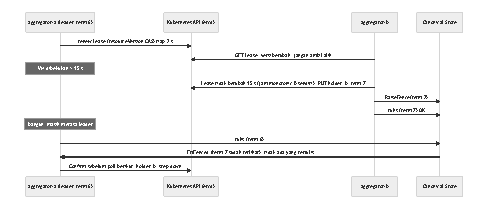
\includegraphics[width=\linewidth,height=0.82\textheight,keepaspectratio]{fig/m4.pdf}\end{figure}

\begin{enumerate}
\item \textbf{Satu penulis lewat leader election} (\texttt{services/\allowbreak{}aggregator/\allowbreak{}internal/\allowbreak{}leader}). Semua instance melayani baca, hanya pemegang Lease \texttt{aggregator-\allowbreak{}ingest} yang menjalankan polling BMKG/PVMBG, relay outbox, dan retry dead letter. Implementasinya klien REST kecil ke API Kubernetes (tanpa client-go): \texttt{GET}, lalu \texttt{POST}/\texttt{PUT} dengan \texttt{resource\allowbreak{}Version} sebagai \emph{compare-and-swap}, sehingga etcd yang mengurutkan semua perubahan.
\item \textbf{Term = token fencing.} Setiap pergantian pemegang menaikkan \texttt{lease\allowbreak{}Transitions}. Konteks kerja leader membawa \texttt{ports.\allowbreak{}Fence\{Name,\allowbreak{} Term,\allowbreak{} Holder\}} dan setiap tulis ke store (\texttt{Save}, \texttt{Set\allowbreak{}Cursor}, dead letter, status sumber) memeriksanya \textbf{di dalam transaksi yang sama} dengan tulisnya (\texttt{adapters/\allowbreak{}postgres/\allowbreak{}unprocessed.\allowbreak{}go}, \texttt{check\allowbreak{}Fence}): baris \texttt{fence} dikunci, term yang lebih kecil dari yang tersimpan ditolak (\texttt{Err\allowbreak{}Fenced}, transaksi di-\emph{rollback}), term yang lebih besar menaikkan nilai tersimpan. Leader baru memanggil \texttt{Raise\allowbreak{}Fence} sebelum tulis pertamanya, karena kunci baris, tulis term lama yang sedang berjalan selesai lebih dulu, dan setiap tulis term lama sesudahnya ditolak.
\item \textbf{Gerbang sebelum memanggil upstream} (\texttt{Loop.\allowbreak{}Gate} = \texttt{Elector.\allowbreak{}Confirm}): sebelum setiap siklus poll, leader membaca ulang Lease. Leader yang baru bangun dari \emph{freeze} langsung tahu ia sudah diganti dan mundur, jadi BMKG/PVMBG tidak menerima permintaan dari dua instance. Header \texttt{X-\allowbreak{}Caller} (nama pod) membuat hal ini terlihat di log upstream.
\item \textbf{Status sumber dibagi lewat store} (\texttt{Put\allowbreak{}Source\allowbreak{}Status}): instance yang tidak polling tetap memberi \texttt{freshness} yang benar. Umur status diukur dengan jam store, status yang tidak diperbarui > 30 s ditandai \texttt{unknown} + \texttt{stale\_\allowbreak{}since}.
\item \textbf{Titik masuk dan rolling update} (\texttt{deploy/\allowbreak{}k8s/\allowbreak{}aggregator.\allowbreak{}yaml}): Service Kubernetes di depan $\ge$ 3 replika dengan \texttt{topology\allowbreak{}Spread\allowbreak{}Constraints} (maxSkew 1 per node), \texttt{readiness\allowbreak{}Probe /\allowbreak{}ready} tiap 2 s (instance yang tidak bisa menjangkau store keluar dari Service setelah 4 s), \texttt{max\allowbreak{}Unavailable: 0}, \texttt{pre\allowbreak{}Stop sleep 10}, dan \emph{graceful shutdown}: permintaan yang sedang berjalan diselesaikan (konteks request tidak ikut dibatalkan SIGTERM), leader melepas Lease saat berhenti sehingga penggantinya mengambil alih dalam $\pm$2 s, bukan 15 s.
\end{enumerate}

\section{Sumber kebenaran waktu (jawaban hint)}

\textbf{Tidak ada jam yang dipercaya untuk keselamatan (safety).} Keputusan ``siapa boleh menulis'' diambil oleh store dari urutan term, bukan dari waktu. Waktu hanya dipakai untuk \textbf{liveness} (kapan mengambil alih), dan itu pun tanpa membandingkan jam dua mesin:


\begin{itemize}
\item Urutan perubahan Lease ditentukan oleh etcd (\texttt{resource\allowbreak{}Version}), satu tempat.
\item Kandidat menganggap Lease kedaluwarsa bila objek Lease \textbf{tidak berubah} selama \texttt{LEASE\_\allowbreak{}DURATION\_\allowbreak{}SEC} menurut \textbf{jam monotonic kandidat sendiri}, dihitung sejak ia pertama kali melihat versi itu. \texttt{renew\allowbreak{}Time} di objek (ditulis dengan jam dinding pemegang) tidak pernah dibaca untuk keputusan. Jam dinding yang melompat +45 s / --30 s tidak menggeser jam monotonic.
\item Leader berhenti sendiri bila gagal memperbarui selama \texttt{RENEW\_\allowbreak{}DEADLINE} (10 s) < \texttt{LEASE\_\allowbreak{}DURATION} (15 s), lagi-lagi dengan jam monotonic-nya. Selisih 5 s itu memastikan, selama laju jam kedua mesin wajar, leader lama sudah berhenti sebelum penerus boleh mengambil alih.
\item Bila asumsi itu dilanggar (VM dibekukan: jam monotonic tidak berjalan), \textbf{fencing} di store tetap mencegah tulis ganda. Waktu tulis untuk audit (\texttt{outbox.\allowbreak{}stored\_\allowbreak{}at}) diambil dari jam store, satu jam untuk semua penulis.
\end{itemize}

Kenapa aman pada kriteria 4: pergeseran jam tidak mengubah keputusan siapa pun (lihat \texttt{Test\allowbreak{}Skewed\allowbreak{}Holder\allowbreak{}Clock\allowbreak{}Does\allowbreak{}Not\allowbreak{}Cause\allowbreak{}Takeover}, \texttt{Test\allowbreak{}Clock\allowbreak{}Jump\allowbreak{}On\allowbreak{}Leader\allowbreak{}Node\allowbreak{}Keeps\allowbreak{}Single\allowbreak{}Leader}). Kenapa aman pada kriteria 5: leader yang bangun memegang term lama, penerusnya sudah menaikkan fence, jadi semua tulisnya ditolak store, dan \texttt{Confirm} membuatnya mundur sebelum poll berikutnya (\texttt{Test\allowbreak{}Frozen\allowbreak{}Leader\allowbreak{}Is\allowbreak{}Fenced\allowbreak{}After\allowbreak{}Waking\allowbreak{}Up}, di cluster: \texttt{scripts/\allowbreak{}demo/\allowbreak{}m2-\allowbreak{}freeze.\allowbreak{}sh} memeriksa \texttt{SELECT count(*) FROM outbox WHERE writer\_\allowbreak{}term =\allowbreak{} <term lama> AND stored\_\allowbreak{}at > <awal freeze>} = 0).


\section{Batas waktu dan trade-off}

{\small
\begin{longtable}{@{}>{\raggedright\arraybackslash}p{0.173\linewidth}>{\raggedright\arraybackslash}p{0.179\linewidth}>{\raggedright\arraybackslash}p{0.582\linewidth}@{}}
\toprule
\textbf{Parameter} & \textbf{Nilai} & \textbf{Alasan dan trade-off} \\
\midrule
\endhead
\texttt{LEASE\_\allowbreak{}DURATION\_\allowbreak{}SEC} & 15 s & Waktu ambil alih terburuk $\approx$ 15 s + 2 s (retry) + 3 s (siklus poll) $\approx$ 20 s, jauh di bawah 60 s. Lebih kecil = failover lebih cepat tetapi jeda GC / jaringan sesaat bisa memicu pergantian leader yang tidak perlu. \\
\texttt{LEASE\_\allowbreak{}RENEW\_\allowbreak{}DEADLINE\_\allowbreak{}SEC} & 10 s & Leader menyerah 5 s sebelum orang lain boleh mengambil alih: margin untuk perbedaan laju jam. \\
\texttt{LEASE\_\allowbreak{}RETRY\_\allowbreak{}PERIOD\_\allowbreak{}SEC} & 2 s & 5 kali kesempatan renew dalam satu deadline, beban API server $\approx$ 1 permintaan / 2 s per instance. \\
\texttt{Confirm} sebelum tiap poll & 1 GET Lease / siklus / sumber & Biaya kecil, menutup celah ``bangun lalu langsung memanggil upstream''. \\
Toleransi node \texttt{unreachable} & 20 s & Pod di node mati diganti setelah 20 s (bawaan 300 s). Terlalu kecil = pod dipindah karena gangguan jaringan singkat. \\
\texttt{SOURCE\_\allowbreak{}STATUS\_\allowbreak{}MAX\_\allowbreak{}AGE\_\allowbreak{}SEC} & 30 s & > durasi lease + beberapa siklus, status yang lebih tua berarti tidak ada yang polling. \\
readiness & tiap 2 s, gagal 2$\times$ & Instance tidak sehat keluar dari Service dalam $\pm$4 s. \\
\bottomrule
\end{longtable}
}

\section{Alternatif yang dipertimbangkan}

{\small
\begin{longtable}{@{}>{\raggedright\arraybackslash}p{0.429\linewidth}>{\raggedright\arraybackslash}p{0.517\linewidth}@{}}
\toprule
\textbf{Alternatif} & \textbf{Ditolak karena} \\
\midrule
\endhead
Lock di PostgreSQL (\texttt{pg\_\allowbreak{}try\_\allowbreak{}advisory\_\allowbreak{}lock} / tabel lease dengan \texttt{now()} DB) & Mengikat koordinasi ke store yang di M2 di-\emph{shard} dan node-nya boleh mati (P1), Lease di etcd hidup di control plane yang tidak dimatikan skenario. \\
client-go \texttt{leaderelection} & Benar secara konsep, tetapi menambah dependensi besar, perilakunya sama (CAS + jam monotonic). Kami tetap butuh fencing karena client-go sendiri menyatakan tidak menjamin satu leader saat proses dijeda. \\
Partisi kerja per sumber tanpa leader (hash sumber ke instance) & Tetap perlu kesepakatan keanggotaan, rebalancing saat skala 3 $\rightarrow$ 5 $\rightarrow$ 2 menimbulkan periode dua pemilik. \\
Idempotensi saja (biarkan tiga instance polling, dedup di store) & Store memang idempoten (hazard\_id deterministik), tetapi upstream menerima permintaan berlipat (dilarang kriteria 2) dan versi hazard bisa saling timpa. \\
\bottomrule
\end{longtable}
}

\section{Batasan yang disadari}

\begin{itemize}
\item Fencing hanya melindungi unit penyimpanan yang \textbf{sudah melihat} term baru. \texttt{Raise\allowbreak{}Fence} menaikkan fence di ketiga shard sebelum tulis pertama, dan setiap tulisan memeriksa fence di transaksinya sendiri (\texttt{repotest} \texttt{run\allowbreak{}Fence} dijalankan untuk adapter \texttt{sharded}).
\item Permintaan HTTP yang \textbf{sudah terkirim} ke upstream tepat sebelum proses dibekukan bisa selesai setelah penerus mulai, hasilnya tetap ditolak store. Log upstream mencatat waktu selesai, jadi yang dibuktikan adalah tidak ada dua caller yang aktif bersamaan setelah serah terima (lihat skrip \texttt{m2-\allowbreak{}single-\allowbreak{}writer.\allowbreak{}sh}).
\item \textbf{Kapasitas cluster demo untuk load test.} Kedua VM dan generator beban (k6) berbagi satu laptop (i5-12500H, 24 GB). Pada 3.000--10.000 VU, node-a, yang sekaligus control plane, jenuh CPU dan API server tidak menjawab. Load test kriteria 6--7 karena itu belum terbukti di perangkat keras ini. Agar sahih, pengujian ini membutuhkan generator beban di mesin lain dan control plane yang tidak ikut melayani beban aplikasi (taint \texttt{No\allowbreak{}Schedule} di node-a, atau node ketiga). Mekanisme yang diuji (scale Deployment, readiness, admisi per peran) sudah dibuktikan terpisah: rolling update di bawah beban (kriteria 8) dan prioritas Lapangan di P5.
\item Lease bergantung pada control plane. Pada topologi 2 node, kehilangan control plane menghentikan pergantian leader (bukan layanan baca). Skenario wajib hanya mematikan worker.
\item Relay outbox hanya di leader, selama serah terima ($\le$ 20 s) event menunggu di outbox, tidak hilang.
\item Polling BMKG/PVMBG memakai \emph{cursor} waktu dengan overlap 5 s (pola M1). Bila sebuah upstream di-restart lalu membuat data baru yang \textbf{bertanggal lebih tua} dari cursor tersimpan, data itu tidak terambil. Contohnya mock BMKG yang membuat 24 event seed mundur hingga 36 jam. Ini bukan celah akibat pergantian leader, karena cursor tersimpan di store dan diteruskan oleh leader berikutnya. Pemeriksaan ``tanpa celah'' di \texttt{m2-\allowbreak{}p2.\allowbreak{}sh} karena itu menilai jendela failover (event sejak 15 menit sebelum leader dimatikan). Perbaikan yang lebih kuat: deteksi restart upstream (prefix ID baru) lalu reset cursor.
\item \textbf{Commit yang sedang berjalan saat freeze.} Pada run pertama di storage sharded, dua baris term 60 tersimpan pada 13:44:49 dan 13:44:54, sesudah pod leader dibekukan (log terakhirnya 13:44:45). Keduanya adalah commit yang sudah terkirim sebelum freeze dan menunggu standby sinkron di node-b yang ikut beku. Commit itu selesai setelah Patroni mencabut status sinkron standby tersebut, dan masih \textbf{sebelum} term 61 menulis pertama kali (13:46:15). Ini tidak melanggar jaminan ``satu penulis per periode''. Pemeriksaan di \texttt{m2-\allowbreak{}freeze.\allowbreak{}sh} karena itu memakai properti yang sebenarnya: tidak ada baris term lama yang tersimpan setelah term baru menulis, pada jam shard yang sama.
\item Selama node dibekukan, API k3s di laptop ini kadang lambat, sehingga pengambilalihan bisa lebih lama dari 15 s. Ini keterbatasan virtualisasi bersarang, bukan logika lease.
\end{itemize}

\section{Bukti per kriteria}

{\small
\begin{longtable}{@{}>{\raggedright\arraybackslash}p{0.161\linewidth}>{\raggedright\arraybackslash}p{0.785\linewidth}@{}}
\toprule
\textbf{Kriteria} & \textbf{Bukti} \\
\midrule
\endhead
1 & \texttt{make demo-\allowbreak{}m2-\allowbreak{}p2} langkah 1 (\texttt{docs/\allowbreak{}evidence/\allowbreak{}m2/\allowbreak{}p2-\allowbreak{}latest.\allowbreak{}log}, k3s 2 VM, storage sharded, 22 Nov): 3 instance di 2 node (\texttt{topology\allowbreak{}Spread\allowbreak{}Constraints max\allowbreak{}Skew=\allowbreak{}1}), Service hanya mengarah ke endpoint Ready. lulus \\
2 & langkah 2--4: tepat satu leader, log BMKG/PVMBG per \texttt{caller} (header \texttt{X-\allowbreak{}Caller}) hanya berurutan per masa kepemimpinan dan tidak pernah tumpang tindih, tidak ada \texttt{(source,\allowbreak{} source\_\allowbreak{}ref\_\allowbreak{}id)} ganda di ketiga shard. lulus \\
3 & langkah 5--6: pod leader dihapus paksa (tanpa melepas lease), penerus melanjutkan ingest \textbf{31 s} setelah kill (lease 15 s, + jadwal poll), 98 event BMKG di jendela failover semuanya tersimpan (missing 0), tanpa duplikat. lulus (bukti 14 Nov dengan store tunggal: 13 s) \\
4 & \texttt{practice clock-\allowbreak{}skew} + \texttt{m2-\allowbreak{}single-\allowbreak{}writer.\allowbreak{}sh}: periode tulis per term (jam store) tidak tumpang tindih \\
5 & \texttt{m2-\allowbreak{}freeze.\allowbreak{}sh} (VM node-b di-\emph{pause} VirtualBox 40 s, storage sharded, 22 Nov, \texttt{docs/\allowbreak{}evidence/\allowbreak{}m2/\allowbreak{}freeze.\allowbreak{}log}): leader term 62 di node-b dibekukan, penerus mengambil lease dengan term 63. Setelah bangun: \textbf{0} baris term 62 tersimpan setelah term 63 menulis (diukur dengan jam masing-masing shard), \textbf{0} log \texttt{hazard\_\allowbreak{}stored} dari pod yang bangun setelah momen freeze, \texttt{m2-\allowbreak{}single-\allowbreak{}writer.\allowbreak{}sh}: tidak ada dua instance yang polling atau menyimpan pada periode yang sama. lulus \\
6 & \texttt{scripts/\allowbreak{}loadtest/\allowbreak{}m2-\allowbreak{}scale.\allowbreak{}sh} dijalankan di cluster demo (k6 v1.4.2 di laptop host, lewat NIC host-only ke NodePort kedua node). \textbf{Tidak tercapai di perangkat keras ini.} Tiga percobaan: 10.000 VU dengan jeda 1 s, 10.000 VU dengan jeda 8 s, dan 3.000 VU dengan jeda 3 s. Semuanya membuat node-a (control plane + worker, 4 vCPU) jenuh. API server berhenti menjawab (\texttt{TLS handshake timeout}), sehingga \texttt{kubectl scale} 3 $\rightarrow$ 5 gagal dan sebagian besar permintaan \emph{timeout} (12.678 permintaan gagal pada percobaan 3.000 VU). Transkrip: \texttt{docs/\allowbreak{}evidence/\allowbreak{}m2/\allowbreak{}p2-\allowbreak{}loadtest-\allowbreak{}scale-\allowbreak{}10k-\allowbreak{}attempt.\allowbreak{}log}. Lihat §6. \\
7 & \texttt{scripts/\allowbreak{}loadtest/\allowbreak{}m2-\allowbreak{}throughput.\allowbreak{}sh} siap (mode \emph{max}, CPU limit sama per pod, 1 lalu 3 instance). Pengukuran di cluster demo \textbf{tidak dilakukan} karena cluster yang sama sudah jenuh pada kriteria 6. Hasilnya tidak akan mengukur Aggregator, melainkan batas CPU laptop yang dipakai bersama oleh k6, kedua VM, dan control plane. \\
8 & langkah 8: \texttt{kubectl set image} \texttt{aggregator:22c2a80} $\rightarrow$ \texttt{aggregator:b500253} di bawah beban paralel: 204 permintaan, \textbf{0 gagal} (\texttt{max\allowbreak{}Unavailable: 0}, preStop, drain, lease dilepas saat SIGTERM). Bukti sebelumnya (14 Nov): 1 955 permintaan, 0 gagal. lulus \\
\bottomrule
\end{longtable}
}

\section{Konfigurasi load testing (Orang 2, butir ``Di laporan'' 4)}

\textbf{Tooling.} k6 (\texttt{grafana/\allowbreak{}k6:0.\allowbreak{}54.\allowbreak{}0}, atau binary \texttt{k6}) dijalankan \textbf{di luar pod aplikasi} (Lampiran B), dari mesin yang menjalankan skrip, ke NodePort Client-Facing API (\texttt{:30080}) \textbf{di setiap node}. VU dibagi rata ke node-node itu sehingga pintu masuk tidak menjadi satu titik.


\textbf{Jalur yang di-scale.} Ingest selalu oleh satu leader, sehingga yang diuji adalah jalur baca:


\begin{lstlisting}
k6 → client-api → Service aggregator → /internal/hazards → store
\end{lstlisting}

Setiap VU adalah klien sungguhan: ia login sekali (\texttt{POST /\allowbreak{}v1/\allowbreak{}token}) lalu memperbarui token sebelum kedaluwarsa (\texttt{/\allowbreak{}v1/\allowbreak{}refresh}), dan memutar empat query \texttt{GET /\allowbreak{}v1/\allowbreak{}hazards} (semua, SEISMIC, VOLCANIC, SIAGA, \texttt{limit=\allowbreak{}20}).


\textbf{Klasifikasi.}


{\small
\begin{longtable}{@{}>{\raggedright\arraybackslash}p{0.160\linewidth}>{\raggedright\arraybackslash}p{0.786\linewidth}@{}}
\toprule
\textbf{Respons} & \textbf{Arti} \\
\midrule
\endhead
200 & berhasil \\
429 & \textbf{penolakan terkontrol} oleh kontrol admisi (Media lebih dulu, \texttt{Retry-\allowbreak{}After}) \\
lainnya & \textbf{error}: 5xx, 401/403, timeout 10 s, gagal koneksi. Ambang k6: \texttt{unhandled rate < 0.\allowbreak{}01} \\
\bottomrule
\end{longtable}
}

\textbf{Kriteria 6} (\texttt{scripts/\allowbreak{}loadtest/\allowbreak{}m2-\allowbreak{}scale.\allowbreak{}sh}):


{\small
\begin{longtable}{@{}>{\raggedright\arraybackslash}p{0.271\linewidth}>{\raggedright\arraybackslash}p{0.675\linewidth}@{}}
\toprule
\textbf{Parameter} & \textbf{Nilai} \\
\midrule
\endhead
VU & \texttt{K6\_\allowbreak{}VUS=\allowbreak{}10000}, \texttt{ramping-\allowbreak{}vus}: naik 30 s $\rightarrow$ tahan 150 s $\rightarrow$ turun 10 s \\
Jeda per iterasi & \texttt{K6\_\allowbreak{}THINK\_\allowbreak{}S=\allowbreak{}1} $\times$ acak 0,5--1,5 \\
Campuran klien & \texttt{K6\_\allowbreak{}MEDIA\_\allowbreak{}SHARE=\allowbreak{}0.\allowbreak{}9}: 90 \% VU Media, 10 \% Tim Lapangan \\
Perubahan instance & \texttt{kubectl scale deploy/\allowbreak{}aggregator} ke 5 pada t = ramp + 30 s, ke 2 pada t = ramp + 90 s (keduanya di tengah fase tahan) \\
Konfigurasi uji (dipulihkan di akhir) & client-api 4 replika dengan laju admisi 2 500 req/s per pod, agar Client-Facing API tidak menjadi yang diukur. Batas \emph{in-flight} tetap 64 per pod, sehingga beban di atas kapasitas menjadi 429 untuk Media, bukan antrean. \\
Pemeriksaan sesudahnya & error rate < 1 \%, lalu \texttt{m2-\allowbreak{}single-\allowbreak{}writer.\allowbreak{}sh} atas jendela uji: tidak ada dua caller upstream yang tumpang tindih, periode tulis per term tidak tumpang tindih, tidak ada HazardEvent ganda \\
\bottomrule
\end{longtable}
}

\textbf{Kriteria 7} (\texttt{scripts/\allowbreak{}loadtest/\allowbreak{}m2-\allowbreak{}throughput.\allowbreak{}sh}): \texttt{K6\_\allowbreak{}MODE=\allowbreak{}max}, 400 VU tetap tanpa jeda selama 60 s, hanya Tim Lapangan (tidak pernah di-\emph{shed}), dengan pemanasan 15 s setelah semua pod Ready. Dijalankan dua kali dengan konfigurasi identik, yang berbeda hanya jumlah instance Aggregator (1 lalu 3).


\begin{itemize}
\item Setiap pod Aggregator diberi \textbf{limit CPU yang sama} (\texttt{AGG\_\allowbreak{}CPU\_\allowbreak{}LIMIT=\allowbreak{}500m}, Lampiran B membebaskan CPU), supaya ``satu instance'' berarti satu unit kapasitas yang tetap, bukan ``semua core sebuah node''.
\item client-api 4 replika dengan admisi longgar, agar bukan client-api yang menjadi bottleneck.
\item Metrik yang dibandingkan adalah \texttt{throughput\_\allowbreak{}ok\_\allowbreak{}rps} (respons 200 per detik), dan rasio 3/1 harus $\ge$ 2,0.
\end{itemize}

\textbf{Catatan kapasitas mesin.} 10 000 VU membutuhkan sekitar 2--3 GB RAM dan \texttt{ulimit -\allowbreak{}n} tinggi di mesin k6. Laptop yang juga menjalankan kedua VM mungkin tidak sanggup, dalam kasus itu skrip dijalankan dari mesin lain di jaringan yang sama dengan kubeconfig cluster. Validasi kecil di mesin pengembang (compose, 300 VU, mode \emph{max}, 90 \% Media) menghasilkan 0 error, Media 26 730 $\times$ 429, dan Tim Lapangan 1 700 $\times$ 200 tanpa satu pun ditolak (\texttt{docs/\allowbreak{}evidence/\allowbreak{}m2/\allowbreak{}p5-\allowbreak{}compose-\allowbreak{}local.\allowbreak{}log}).


\chapter{Problem 3 --- Surat dari Tetangga (Orang 1: kriteria 1--5; Orang 2: kriteria 6)}

> Draf bagian laporan M2. Bukti: \texttt{make demo-\allowbreak{}m2-\allowbreak{}p3} (\texttt{docs/\allowbreak{}evidence/\allowbreak{}m2/\allowbreak{}p3-\allowbreak{}latest.\allowbreak{}log}), \texttt{make demo-\allowbreak{}p1} (M1, kini > memakai dead-letter store), test \texttt{services/\allowbreak{}aggregator/\allowbreak{}internal/\allowbreak{}\{sources,\allowbreak{}dlq,\allowbreak{}poller,\allowbreak{}mapping,\allowbreak{}api\}}, > \texttt{internal/\allowbreak{}ports/\allowbreak{}repotest} (\texttt{runUnprocessed}), dan \texttt{services/\allowbreak{}pvmbg-\allowbreak{}mock/\allowbreak{}internal/\allowbreak{}pvmbg/\allowbreak{}m2\_\allowbreak{}test.\allowbreak{}go}. > Bagian kriteria 6 (\texttt{POST /\allowbreak{}field-\allowbreak{}reports}) ditulis Orang 2.


\section{Identifikasi masalah}

{\small
\begin{longtable}{@{}>{\raggedright\arraybackslash}p{0.112\linewidth}>{\raggedright\arraybackslash}p{0.411\linewidth}>{\raggedright\arraybackslash}p{0.411\linewidth}@{}}
\toprule
\textbf{Kriteria} & \textbf{Persoalan} & \textbf{Nama dalam literatur} \\
\midrule
\endhead
2 & Pesan yang gagal diproses harus disimpan, bukan dibuang atau dicoba terus-menerus; kegagalan sementara harus dibedakan dari kegagalan permanen & \emph{Dead letter queue / dead letter channel} (Hohpe \& Woolf, \emph{Enterprise Integration Patterns}); \emph{transient vs permanent fault}, \emph{retry with exponential backoff} \\
3 & Satu pesan rusak (terpotong, bersarang sangat dalam, UTF-8 rusak, sangat besar) membuat parser gagal atau proses kehabisan memori, lalu restart berulang dan memblokir pesan lain & \emph{Poison message / poison pill}; \emph{head-of-line blocking}; \emph{crash loop} \\
4 & Setelah sistem disesuaikan, pesan lama diproses ulang: tidak boleh ganda dan tidak boleh menimpa data yang lebih baru & \emph{Replay / reprocessing} dengan \emph{idempotent consumer}; \emph{per-key ordering} (\emph{ordered delivery per entity}) \\
1 & Skema mitra berubah tanpa koordinasi; sistem harus tahu mana yang boleh diterima & \emph{Schema evolution}, \emph{tolerant reader} (Fowler), kompatibilitas \emph{backward/forward} \\
6 & Laporan Tim Lapangan harus diterima walau pemrosesan hilir lambat atau mati, tidak boleh hilang setelah dijawab 202 walau penerimanya mati, dan tidak boleh diproses dua kali walau klien mengulang & \emph{Asynchronous request--reply} / \emph{request acknowledgement} (202 Accepted), \emph{durable message queue} (\emph{store-and-forward}), \emph{at-least-once delivery} + \emph{idempotent receiver} (Hohpe \& Woolf) = \emph{effectively-once}; \emph{exactly-once processing} dengan \emph{transactional consume--transform--produce} (Kafka KIP-98/KIP-447); \emph{zombie fencing} \\
\bottomrule
\end{longtable}
}

\section{Kebijakan perubahan skema (kriteria 1)}

Kebijakan M1 dipertahankan dan dinyatakan di komentar paket \texttt{services/\allowbreak{}aggregator/\allowbreak{}internal/\allowbreak{}mapping/\allowbreak{}raw.\allowbreak{}go}:


{\small
\begin{longtable}{@{}>{\raggedright\arraybackslash}p{0.307\linewidth}>{\raggedright\arraybackslash}p{0.296\linewidth}>{\raggedright\arraybackslash}p{0.331\linewidth}@{}}
\toprule
\textbf{Perubahan} & \textbf{Sikap} & \textbf{Alasan} \\
\midrule
\endhead
Field baru (tipe apa pun) & \textbf{diterima otomatis} $\rightarrow$ \texttt{attributes} & Tidak mengubah arti field kanonik; tidak ada data yang dibuang \\
Field non-kanonik hilang atau berganti tipe & \textbf{diterima otomatis} & Disimpan apa adanya di \texttt{attributes}; tidak ada aturan pemetaan yang bergantung padanya \\
Urutan / format field & \textbf{diterima otomatis} & Record dibaca sebagai peta, bukan posisi \\
Field kanonik di-\emph{rename}, dihapus, dipindah, atau berganti tipe; nilai enum baru & \textbf{tidak diterima} $\rightarrow$ \emph{parked} \texttt{schema\_\allowbreak{}incompatible} & Menebak arti sama dengan risiko severity atau lokasi yang salah pada peringatan bencana \\
Byte yang tidak bisa dibaca & \textbf{tidak diterima} $\rightarrow$ \emph{parked} \texttt{malformed} (\emph{retrying} bila terpotong di jalan) & Tidak ada isi yang bisa dipetakan \\
\bottomrule
\end{longtable}
}

Mock PVMBG mendapat mode baru di \texttt{POST /\allowbreak{}admin/\allowbreak{}schema-\allowbreak{}version} (\texttt{\{"mode":"incompatible"\}} / \texttt{\{"version":3\}} / pilihan \texttt{\{"incompatible":["rename",\allowbreak{}"type\_\allowbreak{}change",\allowbreak{}"drop\_\allowbreak{}required"]\}}): \texttt{alert\_\allowbreak{}level} $\rightarrow$ \texttt{level}, \texttt{reported\_\allowbreak{}at} ISO $\rightarrow$ angka Unix, \texttt{volcano\_\allowbreak{}id} hilang (kodenya pindah ke \texttt{location.\allowbreak{}volcano\_\allowbreak{}code}). Laporan lama tetap berbentuk lama, seperti versi API baru di dunia nyata. \texttt{POST /\allowbreak{}admin/\allowbreak{}malformed} membuat pesan rusak.


\section{Mekanisme}

\begin{figure}[H]\centering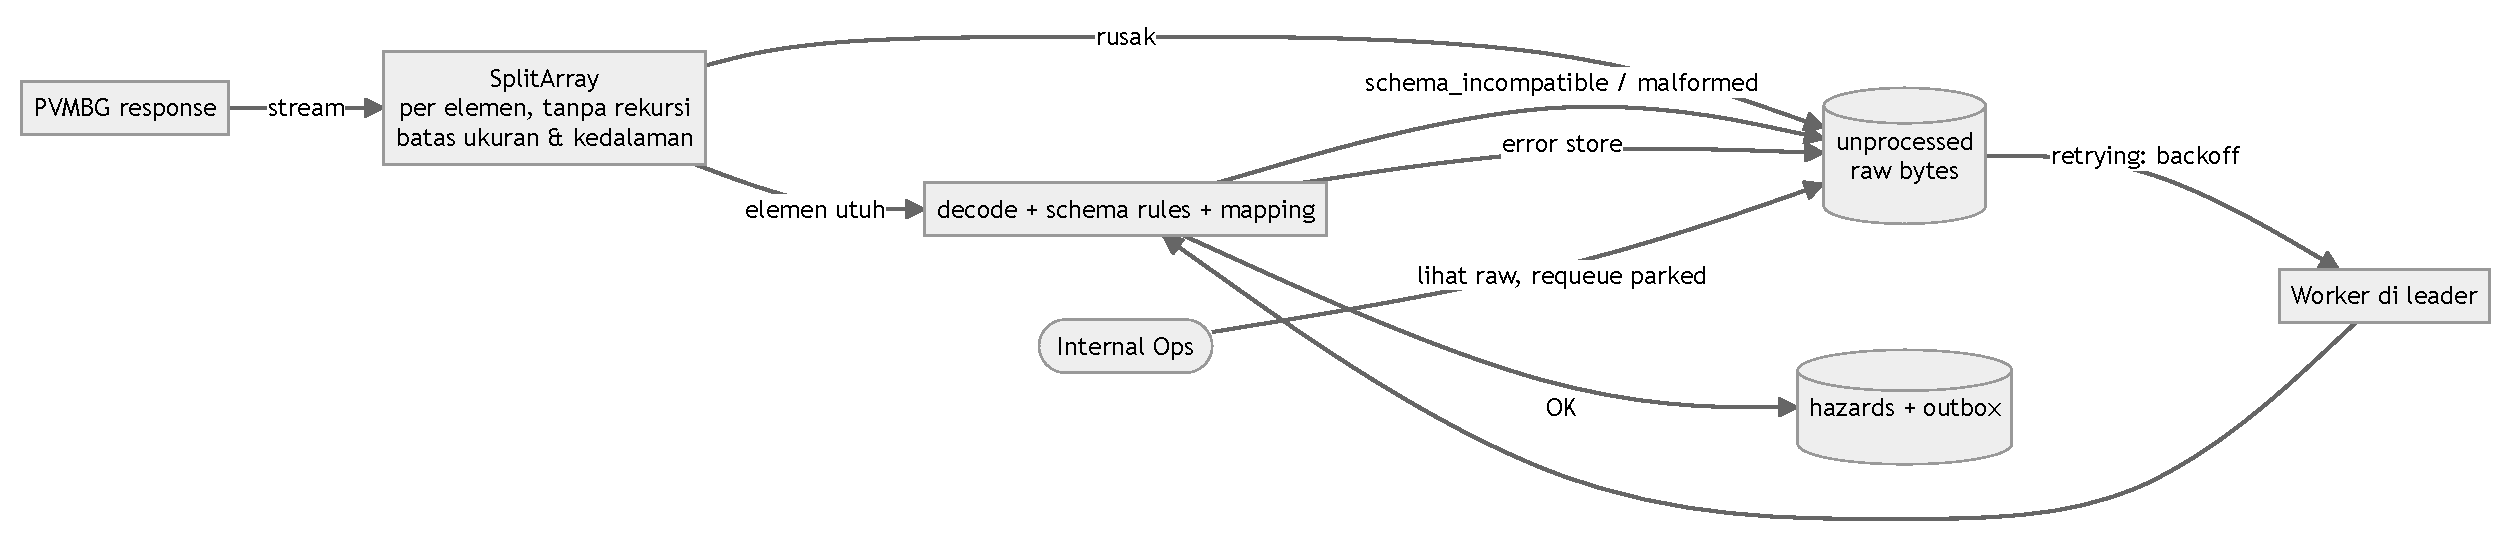
\includegraphics[width=\linewidth,height=0.82\textheight,keepaspectratio]{fig/m5.pdf}\end{figure}

\begin{enumerate}
\item \textbf{Membaca tanpa bisa dijatuhkan} (\texttt{sources/\allowbreak{}split.\allowbreak{}go}). Respons dibaca sebagai \emph{stream} dan dipecah per elemen array tanpa di-\emph{decode}: kedalaman dihitung dengan penghitung (tanpa rekursi), satu elemen paling banyak \texttt{MESSAGE\_\allowbreak{}MAX\_\allowbreak{}BYTES} (1 MiB) ditahan di memori, UTF-8 diperiksa eksplisit (\texttt{encoding/\allowbreak{}json} diam-diam mengganti byte rusak dengan U+FFFD). Elemen rusak dikembalikan bersama masalahnya; elemen di sekitarnya tetap diproses. Tidak ada \texttt{panic} yang mungkin dari input.
\item \textbf{Dead-letter store} (\texttt{internal/\allowbreak{}dlq}, tabel \texttt{unprocessed} di Canonical Store). Setiap pesan gagal disimpan dengan \textbf{byte persis} yang diterima, \texttt{reason}, \texttt{source}, \texttt{received\_\allowbreak{}at}, \texttt{kind}, \texttt{record\_\allowbreak{}key}, \texttt{attempts}, \texttt{status}. \texttt{message\_\allowbreak{}id} = sha256(source, kind, bytes), jadi pesan yang diambil ulang oleh jendela overlap polling tidak tersimpan dua kali.
\item \textbf{Dua perlakuan berbeda} (kriteria 2):
\begin{itemize}
\item \emph{retrying} (\texttt{retryable: true}): kegagalan yang bisa hilang sendiri --- tulis ke store gagal, peringatan tsunami yang event-nya belum datang (\texttt{dependency\_\allowbreak{}missing}), elemen terpotong di jalan (sumber dipoll ulang dari watermark yang sama). Worker di leader mencoba ulang dengan \emph{exponential backoff} 2 s \ldots{} 120 s, maksimum 8 kali, lalu \emph{parked} \texttt{retry\_\allowbreak{}exhausted}. Elemen terpotong selesai sendiri begitu record utuhnya tersimpan.
\item \emph{parked} (\texttt{retryable: false}): \texttt{schema\_\allowbreak{}incompatible} dan \texttt{malformed}. \textbf{Tidak pernah dicoba otomatis} (mencoba lagi byte yang sama dengan kode yang sama pasti gagal). Menunggu perubahan sistem lalu \emph{requeue} oleh Internal Ops.
\end{itemize}
\item \textbf{Watermark tidak tertahan pesan buruk}: kursor polling maju melewati pesan yang sudah aman di dead-letter store, sehingga satu pesan rusak tidak membuat sumber diambil ulang terus (head-of-line blocking).
\item \textbf{Penyesuaian sistem tanpa kode baru} (\texttt{mapping/\allowbreak{}rules.\allowbreak{}go}): aturan deklaratif per sumber --- \texttt{rename} (termasuk path bersarang) dan \texttt{coerce} (\texttt{unix\_\allowbreak{}seconds\_\allowbreak{}to\_\allowbreak{}rfc3339}, \texttt{number\_\allowbreak{}to\_\allowbreak{}string}, \ldots{}) --- dimuat dari ConfigMap \texttt{aggregator-\allowbreak{}schema-\allowbreak{}rules}. Aturan hanya \textbf{mengisi field kanonik yang kosong}, jadi record skema lama tidak berubah. Aturan tidak valid menghentikan start-up (pod tidak Ready, rollout berhenti), bukan diabaikan diam-diam. Contoh penyesuaian PVMBG v3: \texttt{deploy/\allowbreak{}schema-\allowbreak{}rules/\allowbreak{}pvmbg-\allowbreak{}v3.\allowbreak{}json}.
\item \textbf{Pemrosesan ulang} (kriteria 4): \texttt{POST /\allowbreak{}internal/\allowbreak{}ops/\allowbreak{}unprocessed/\allowbreak{}reprocess} memindahkan pesan \emph{parked} ke \emph{retrying}. Worker memprosesnya dengan \textbf{kode yang sama} dengan jalur normal (\texttt{PVMBGSource.\allowbreak{}process}), urut kedatangan (\texttt{seq}).
\begin{itemize}
\item \emph{Tanpa duplikat}: \texttt{hazard\_\allowbreak{}id} deterministik dan \texttt{Upsert} idempoten; pesan yang ternyata sudah tersimpan menghasilkan \texttt{unchanged}.
\item *Urutan per \texttt{source\_\allowbreak{}ref\_\allowbreak{}id}*: selama ada pesan terbuka untuk record yang sama (sumber + kind + \texttt{record\_\allowbreak{}key}), pesan baru record itu ikut masuk antrean dengan alasan \texttt{ordered\_\allowbreak{}after: <id>} dan worker hanya memproses pesan terdepan per record. Pesan lama yang pulih tidak bisa menimpa data yang lebih baru (\texttt{TestIncompatibleChangeRecoversAfterAdjustmentInOrderWithoutDuplicates}: VR-1 v1 diproses sebelum v2, hasil akhir AWAS v2).
\end{itemize}
\item \textbf{Hanya Internal Ops} (kriteria 5): \texttt{/\allowbreak{}internal/\allowbreak{}ops/\allowbreak{}*} hanya menerima \texttt{Authorization: Bearer <AGGREGATOR\_\allowbreak{}OPS\_\allowbreak{}TOKEN>}. Kredensial Client-Facing API (\texttt{X-\allowbreak{}Service-\allowbreak{}Key}) dan token auditor ditolak (401/403). Auditor mendapat \texttt{/\allowbreak{}internal/\allowbreak{}audit/\allowbreak{}unprocessed} (Lampiran A) yang hanya memuat metadata, tanpa isi pesan. \texttt{GET /\allowbreak{}internal/\allowbreak{}quarantine} M1, yang terbuka untuk service key, dihapus.
\end{enumerate}

\section{Alternatif yang dipertimbangkan}

{\small
\begin{longtable}{@{}>{\raggedright\arraybackslash}p{0.297\linewidth}>{\raggedright\arraybackslash}p{0.649\linewidth}@{}}
\toprule
\textbf{Alternatif} & \textbf{Konsekuensi} \\
\midrule
\endhead
Buang pesan buruk dan catat di log & Melanggar kriteria 2; isi tidak bisa diproses ulang \\
DLQ sebagai topic Kafka & Wajar untuk alur push, tetapi butuh konsumen DLQ, penyimpanan status, dan akses terkontrol tambahan; tabel di store yang sudah dimiliki Aggregator memberi query, status, dan transaksi dengan fencing tanpa komponen baru \\
Retry semua kegagalan dengan backoff & Pesan rusak permanen mengisi antrean retry selamanya dan menyamarkan masalah nyata \\
Coba tebak (\texttt{level} mungkin \texttt{alert\_\allowbreak{}level}) & Cepat, tetapi tebakan salah pada peringatan bencana lebih berbahaya daripada keterlambatan; penyesuaian tetap butuh keputusan manusia \\
Parser JSON standar untuk seluruh respons & Satu elemen buruk menggagalkan seluruh batch; kedalaman ekstrem dan ukuran besar memakan memori \\
\bottomrule
\end{longtable}
}

\section{Batasan yang disadari}

\begin{itemize}
\item Pesan melebihi \texttt{MESSAGE\_\allowbreak{}MAX\_\allowbreak{}BYTES} disimpan \textbf{1 MiB pertama} + ukuran aslinya (bukan ``utuh''), agar satu pesan tidak bisa menghabiskan memori atau tabel. Pesan seperti itu tidak bisa dipulihkan dengan aturan skema; perlu perubahan batas.
\item Watermark hanya maju oleh record yang waktunya bisa dibaca. Bila sumber mengubah tipe \texttt{reported\_\allowbreak{}at}, record baru diambil ulang tiap siklus sampai aturan dipasang (tidak ganda karena \texttt{message\_\allowbreak{}id}), dengan biaya bandwidth.
\item Elemen terpotong tanpa \texttt{report\_\allowbreak{}id} yang terbaca tidak bisa dikaitkan dengan record utuhnya; ia di-\emph{parked} \texttt{retry\_\allowbreak{}exhausted} setelah 8 percobaan (datanya sendiri tetap masuk dari respons berikutnya).
\item Aturan skema hanya \texttt{rename} dan \texttt{coerce}. Perubahan makna atau satuan butuh kode baru (versi Aggregator baru, rolling update tanpa downtime, lalu requeue --- jalurnya sama).
\end{itemize}

\section{Bukti per kriteria}

{\small
\begin{longtable}{@{}>{\raggedright\arraybackslash}p{0.161\linewidth}>{\raggedright\arraybackslash}p{0.785\linewidth}@{}}
\toprule
\textbf{Kriteria} & \textbf{Bukti} \\
\midrule
\endhead
1 & \texttt{make demo-\allowbreak{}m2-\allowbreak{}p3} langkah 1 (field baru diterima otomatis ke \texttt{attributes}) dan 4 (3 laporan tidak kompatibel di-\emph{parked} dengan byte persis, tidak ditebak). Diulang 22 Nov di storage sharded: \texttt{p3-\allowbreak{}sharded-\allowbreak{}20261122.\allowbreak{}log}. lulus \\
2 & langkah 2: \texttt{too\_\allowbreak{}deep}, \texttt{invalid\_\allowbreak{}utf8}, \texttt{too\_\allowbreak{}large} \emph{parked} (attempts tidak bertambah), elemen terpotong \emph{retrying} $\rightarrow$ \emph{resolved} sendiri tanpa intervensi (22 Nov, sharded). lulus \\
3 & langkah 2: restart count Aggregator tidak berubah; laporan valid yang dikirim bersama pesan rusak tetap tersimpan (22 Nov, sharded). lulus \\
4 & langkah 5: aturan PVMBG v3 dipasang lewat rolling update, requeue, ketiga laporan tersimpan, \texttt{count(*) -\allowbreak{} count(DISTINCT source\_\allowbreak{}ref\_\allowbreak{}id) =\allowbreak{} 0}. lulus di k3s pada 14 Nov (\texttt{p3-\allowbreak{}latest.\allowbreak{}log}, store tunggal). Pada ulangan 22 Nov di storage sharded, rolling update untuk memasang aturan tidak selesai: pod Aggregator baru tidak dapat menjangkau Kafka karena NetworkPolicy node-a belum menerima IP pod baru setelah node itu di-reset paksa (lihat §5). Langkah ini tidak bergantung pada jenis storage. \\
5 & langkah 3: \texttt{X-\allowbreak{}Service-\allowbreak{}Key} 401, service key sebagai Bearer 403, token audit 403, token Ops 200 (22 Nov, sharded). lulus \\
6 & \texttt{make demo-\allowbreak{}m2-\allowbreak{}field-\allowbreak{}reports} (\texttt{docs/\allowbreak{}evidence/\allowbreak{}m2/\allowbreak{}p3-\allowbreak{}field-\allowbreak{}reports-\allowbreak{}latest.\allowbreak{}log}; run pengembangan: \texttt{p3-\allowbreak{}field-\allowbreak{}reports-\allowbreak{}kind.\allowbreak{}log}): pemroses mati, 20$\times$202 p50 36 ms / p95 298 ms; 5 retry $\rightarrow$ \texttt{report\_\allowbreak{}id} sama; semua pod client-api dibunuh setelah 202; pemroses dibunuh di tengah transaksi; 40 diterima $\rightarrow$ 40 record di \texttt{field-\allowbreak{}reports.\allowbreak{}processed}, 40 berbeda. Test: \texttt{client-\allowbreak{}api/\allowbreak{}internal/\allowbreak{}api/\allowbreak{}fieldreports\_\allowbreak{}test.\allowbreak{}go}, \texttt{field-\allowbreak{}reports/\allowbreak{}internal/\allowbreak{}processor/\allowbreak{}processor\_\allowbreak{}test.\allowbreak{}go} (duplikat, restart, zombie) \\
\bottomrule
\end{longtable}
}

\section{Kriteria 6 --- \texttt{POST /\allowbreak{}field-\allowbreak{}reports} (Orang 2)}

\subsection{Persoalan}

Tim Lapangan mengirim laporan dari lokasi dengan sinyal yang mungkin hanya cukup untuk satu kali kirim. Ada tiga hal yang dapat merusaknya:


\begin{enumerate}
\item \textbf{Hilir lambat atau mati.} Bila 202 menunggu pemrosesan, satu pemroses yang lambat membuat semua pengirim menunggu sampai timeout dan mengulang. Inilah alasan pola \emph{asynchronous request--reply}: terima dulu, proses kemudian.
\item \textbf{Penerima mati setelah 202.} Laporan yang hanya ada di memori proses penerima ikut hilang. Masalah ini disebut \emph{durability before acknowledgement}: yang boleh dijawab ``diterima'' hanyalah yang sudah tersimpan tahan lama.
\item \textbf{Pengiriman ulang.} Jaringan dapat menelan balasan 202. Klien yang benar akan mengirim ulang, dan sistem melihat laporan yang sama dua kali. Jaminan \emph{at-least-once} hanya aman bila penerimanya \emph{idempotent receiver}. Sebaliknya, pemroses yang mati di tengah pekerjaan akan mengulang input yang sudah setengah diproses, dan ini juga memerlukan \emph{exactly-once processing}.
\end{enumerate}

\subsection{Mekanisme}

\begin{lstlisting}
Tim Lapangan --POST + Idempotency-Key--> client-api --produce acks=all--> [field-reports] --202-->
                                                         (idempoten)          |
                       services/field-reports: consume --(transaksi Kafka)--> [field-reports.processed] + commit offset
\end{lstlisting}

\begin{itemize}
\item \textbf{Kunci idempotensi dan identitas laporan.} Klien mengirim \texttt{Idempotency-\allowbreak{}Key}, lalu \texttt{report\_\allowbreak{}id =\allowbreak{} sha256(client\_\allowbreak{}id,\allowbreak{} key)}. Pengulangan dengan kunci yang sama menghasilkan \texttt{report\_\allowbreak{}id} dan key Kafka yang sama, sehingga masuk ke partisi yang sama dengan urutan yang terjaga.
\item \textbf{Tahan lama sebelum 202.} client-api memanggil \texttt{ProduceSync} dengan \texttt{acks=\allowbreak{}all} dan producer idempoten. Producer idempoten mencegah satu produce yang diulang oleh library tertulis dua kali di partisi. 202 baru dikirim setelah broker mengonfirmasi. client-api tidak menyimpan apa pun sesudahnya, jadi pod-nya boleh mati kapan saja. Bila broker tidak menjawab dalam 5 s, klien mendapat 503 dan mengulang dengan kunci yang sama. Pemroses hilir tidak ada di jalur ini: 202 tetap cepat walau pemroses mati (demo langkah 1: p95 0,30 s dengan pemroses 0 replika).
\item \textbf{Pemrosesan exactly-once.} \texttt{services/\allowbreak{}field-\allowbreak{}reports} memakai \texttt{kgo.\allowbreak{}GroupTransactSession}. Dalam \textbf{satu transaksi}, pemroses menulis record hasil ke \texttt{field-\allowbreak{}reports.\allowbreak{}processed} dan meng-commit offset input. Akibatnya:
\begin{itemize}
\item bila pemroses mati sebelum commit, transaksi di-abort, keluaran tidak terlihat oleh pembaca \texttt{read\_\allowbreak{}committed}, dan input dibaca ulang;
\item bila mati sesudah commit, tidak ada yang perlu diulang.
\end{itemize}
\item \textbf{Dedup lintas pengulangan klien.} Laporan yang sama yang dikirim dua kali adalah dua record input. Pemroses menyimpan set \texttt{report\_\allowbreak{}id} yang sudah diproses dan melewati yang kedua. Set ini dibangun ulang saat start dari topic \emph{compacted} \texttt{field-\allowbreak{}reports.\allowbreak{}processed} (read\_committed, sampai \emph{last stable offset}), sebelum bergabung ke group. Karena itu pemroses tidak membutuhkan database sendiri.
\item \textbf{Zombie.} Instance lama yang masih hidup (beku, terpartisi) di-fence dua kali:
\begin{itemize}
\item oleh \texttt{transactional.\allowbreak{}id} yang sama, karena instance baru menaikkan epoch sehingga commit instance lama ditolak \texttt{PRODUCER\_\allowbreak{}FENCED};
\item oleh generasi consumer group, karena commit offset instance lama ditolak setelah rebalance.

Setiap batch yang gagal mengakhiri sesi; sesi baru (epoch baru) dibuat setelah set dedup dibangun ulang. Test
\texttt{TestZombieIsFencedAndNothingIsProcessedTwice} membuktikannya.
\end{itemize}
\end{itemize}

\subsection{Jaminan pengiriman (butir ``Di laporan'' 4)}

\emph{*At-least-once dari klien ke broker, exactly-once dari broker ke hasil olahan, jadi *effectively exactly-once} per \texttt{report\_\allowbreak{}id}.** Rinciannya:


\begin{itemize}
\item Laporan yang mendapat 202 sudah ada di log Kafka yang tahan lama, sehingga \textbf{tidak hilang} walau client-api atau pemroses mati.
\item Laporan yang tidak mendapat 202 menjadi tanggung jawab klien: ia mengulang dengan kunci yang sama.
\item Setiap \texttt{report\_\allowbreak{}id} muncul \textbf{tepat sekali} di \texttt{field-\allowbreak{}reports.\allowbreak{}processed} (read\_committed).
\end{itemize}

Bukti (\texttt{make demo-\allowbreak{}m2-\allowbreak{}field-\allowbreak{}reports}):


\begin{enumerate}
\item Pemroses di-\emph{scale} ke 0; 20 laporan semuanya 202 (p95 0,30 s).
\item Lima laporan dikirim ulang dengan kunci sama; \texttt{report\_\allowbreak{}id} tetap sama.
\item Semua pod client-api dibunuh (\texttt{-\allowbreak{}-\allowbreak{}grace-\allowbreak{}period=\allowbreak{}0 -\allowbreak{}-\allowbreak{}force}) tepat setelah 20 laporan berikutnya mendapat 202.
\item Pemroses dihidupkan dengan jeda 300 ms per laporan, lalu dibunuh di tengah transaksi.
\item Topic hasil berisi **40 record untuk 40 \texttt{report\_\allowbreak{}id} berbeda**, sama dengan jumlah \texttt{report\_\allowbreak{}id} yang mendapat 202. Log memperlihatkan \texttt{dedup\_\allowbreak{}set\_\allowbreak{}rebuilt} dan \texttt{field\_\allowbreak{}report\_\allowbreak{}duplicate\_\allowbreak{}skipped} untuk retry.
\end{enumerate}

\subsection{Alternatif}

{\small
\begin{longtable}{@{}>{\raggedright\arraybackslash}p{0.321\linewidth}>{\raggedright\arraybackslash}p{0.625\linewidth}@{}}
\toprule
\textbf{Alternatif} & \textbf{Konsekuensi} \\
\midrule
\endhead
Proses sinkron lalu jawab 200 & 202 tidak lagi cepat ketika hilir lambat atau mati; klien timeout dan mengulang sehingga beban berlipat. Ditolak. \\
Antrean di memori client-api (channel) lalu 202 & Laporan hilang bila pod mati setelah 202. Melanggar kriteria. \\
Tulis ke database client-api lalu \emph{outbox} & Benar, tetapi client-api butuh storage sendiri (aturan satu storage satu pemilik, PV, backup), padahal Kafka sudah tahan lama dan sudah dipakai. \\
Consumer at-least-once + dedup di database & Dedup tetap butuh storage, dan ada celah antara ``tulis hasil'' dan ``commit offset''. Transaksi Kafka menutup celah itu tanpa storage tambahan. \\
Dedup di client-api (cek kunci sebelum produce) & client-api stateless dengan banyak replika; dedup di sana butuh state bersama dan tetap racy. Dedup di pemroses (satu writer per partisi) cukup dan sederhana. \\
\bottomrule
\end{longtable}
}

\subsection{Batasan yang disadari}

\begin{itemize}
\item Broker Kafka satu node (\texttt{replication.\allowbreak{}factor=\allowbreak{}1}, keputusan M1). \texttt{acks=\allowbreak{}all} berarti ditulis ke log broker. Bila disk node broker hilang, laporan yang belum diproses ikut hilang. Replikasi broker ($\ge$ 3 broker) adalah perbaikan berikutnya dan di luar kapasitas cluster 2 VM.
\item Set dedup ada di memori pemroses dan dibangun ulang dari topic compacted. Waktu start sebanding dengan jumlah \texttt{report\_\allowbreak{}id} unik (kecil untuk PoC).
\item Kunci yang sama dengan isi berbeda diperlakukan sebagai pengulangan: isi pertama yang menang. Ini tidak dideteksi sebagai konflik.
\item \texttt{GET /\allowbreak{}v1/\allowbreak{}field-\allowbreak{}reports/\allowbreak{}\{id\}} hanya mengenal laporan yang \textbf{sudah diproses}. Laporan yang diterima tetapi belum diproses menghasilkan 404 sampai diproses.
\end{itemize}

\chapter{Problem 4: Atap Seng di Siang Bolong}

\section{Identifikasi masalah (butir ``Di laporan'' 1)}

{\small
\begin{longtable}{@{}>{\raggedright\arraybackslash}p{0.224\linewidth}>{\raggedright\arraybackslash}p{0.355\linewidth}>{\raggedright\arraybackslash}p{0.355\linewidth}@{}}
\toprule
\textbf{Kriteria} & \textbf{Persoalan yang sebenarnya terjadi} & \textbf{Nama dan konsep dalam literatur} \\
\midrule
\endhead
2. Pengelompokan menurut waktu deteksi, keterlambatan & Data tiba tidak berurutan dan terlambat. Urutan tiba di BNPB tidak sama dengan urutan lintasan satelit, dan sebagian laporan lintasan pagi baru tiba siang. Pengelompokan yang memakai waktu tiba akan memisahkan deteksi yang seharusnya satu kebakaran. & \emph{Event time vs processing time}, \emph{out-of-order / late data}, \textbf{watermark} dan \emph{allowed lateness} (Dataflow Model, Akidau dkk. 2015, Streaming Systems). Pengelompokan berdasarkan kedekatan ruang dan waktu adalah \emph{session-like windowing} atas graf (\emph{connected components}, mirip DBSCAN dengan \texttt{min\allowbreak{}Pts =\allowbreak{} 2}). \\
4. Lonjakan 60$\times$, tanpa kehilangan, kembali mutakhir $\le$ 60 s & Laju masuk sesaat melebihi laju olah. Bila tidak ada buffer yang tahan lama dan posisi baca yang tersimpan, data hilang atau sistem tertinggal tanpa terlihat. & \emph{Backpressure}, \textbf{consumer lag}, \emph{log-based messaging} dengan offset (Kleppmann, DDIA bab 11), \emph{catch-up} setelah \emph{burst}. \\
5. Pemroses mati di tengah pengenalan kebakaran & Keadaan sementara (anggota graf, ID kebakaran, mutasi yang belum diterapkan) hilang bila hanya ada di memori. Pengulangan setelah restart juga bisa menggandakan hasil. & \textbf{Exactly-once processing / effectively-once}: \emph{checkpointing} keadaan bersama offset (Chandy--Lamport, Flink), \textbf{idempotent sink} dengan versi, \emph{at-least-once delivery + deduplication}. \\
\bottomrule
\end{longtable}
}

\section{Mengapa polling M1 ditinggalkan untuk sumber ini (butir ``Di laporan'' 2)}

Pola M1 adalah \emph{polling} dengan \emph{cursor} waktu dan \emph{overlap}. Pola ini cocok untuk BMKG dan PVMBG: datanya sedikit, setiap record berdiri sendiri, dan pengambilan ulang dengan overlap aman karena upsert idempoten. Untuk Feed Satelit pola itu ditinggalkan, karena:


\begin{enumerate}
\item \textbf{Feed sudah berupa log berurutan.} Setiap kejadian punya offset yang naik monoton tanpa celah, dan stream dapat dilanjutkan dengan \texttt{from=\allowbreak{}<offset>} atau \texttt{Last-\allowbreak{}Event-\allowbreak{}ID}. Posisi baca yang tepat adalah satu bilangan. Cursor waktu tidak bisa menangkap \texttt{update} dan \texttt{retract}, karena keduanya merujuk ke deteksi lama.
\item \textbf{Lonjakan ribuan deteksi per lintasan.} Polling setiap beberapa detik menambah latensi sebesar interval dan membuang permintaan saat feed diam. SSE mendorong data begitu tersedia. Heartbeat memberi tanda hidup dan ikut memajukan offset.
\item \textbf{Batas koneksi.} Feed menolak koneksi berlipat (\texttt{429 too\_\allowbreak{}many\_\allowbreak{}connections}). Dengan satu koneksi SSE milik leader ingest (mekanisme P2), feed hanya dibaca sekali oleh seluruh sistem.
\end{enumerate}

Yang \textbf{dipertahankan} dari M1: satu penulis ber-fencing (lease Kubernetes, P2), penyimpanan idempoten dengan versi, dan outbox $\rightarrow$ Kafka untuk konsumen hilir.


\section{Rancangan}

\begin{figure}[H]\centering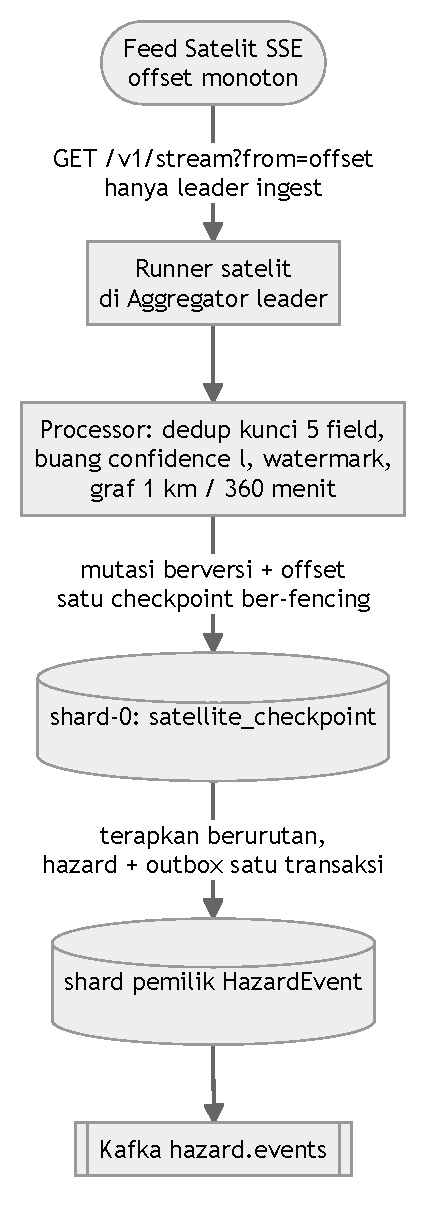
\includegraphics[width=\linewidth,height=0.82\textheight,keepaspectratio]{fig/m6.pdf}\end{figure}

\subsection{Dari deteksi ke HazardEvent WILDFIRE (kriteria 1, 3)}

\begin{itemize}
\item \textbf{Identitas deteksi.} Kunci \texttt{satellite|\allowbreak{}acq\_\allowbreak{}date|\allowbreak{}acq\_\allowbreak{}time|\allowbreak{}latitude|\allowbreak{}longitude} diambil \emph{apa adanya} dari teks feed, termasuk nol di depan dan di belakang. Untuk perhitungan, waktu dan koordinat di-parse terpisah. Deteksi dengan kunci sama yang tiba ulang diabaikan.
\item \textbf{Waktu deteksi} adalah \texttt{acq\_\allowbreak{}date + acq\_\allowbreak{}time} dalam UTC, bukan waktu tiba.
\item **Confidence \texttt{l}\emph{* tidak ikut dikelompokkan. Deteksinya tetap disimpan sebagai *inactive}, supaya \texttt{update} yang menaikkan confidence-nya tetap bisa diterapkan.
\item \textbf{Keterhubungan.} Dua deteksi terhubung bila jaraknya $\le$ 1,0 km (haversine) \textbf{dan} selisih waktunya $\le$ 360 menit. Calon tetangga dicari lewat grid sel ECEF 1 km $\times$ 6 jam, lalu jarak dihitung tepat. Komponen terhubung (BFS) dengan $\ge$ 2 deteksi menjadi satu kebakaran, termasuk bila deteksinya dari satelit berbeda. Deteksi tunggal dihitung dan dilaporkan (\texttt{singletons}).
\item \textbf{Pemetaan.} \texttt{occurred\_\allowbreak{}at} = deteksi paling awal, \texttt{latitude/\allowbreak{}longitude} = centroid sferis, \texttt{area\_\allowbreak{}name} = provinsi dengan titik pusat terdekat pada tabel statis (\texttt{SATELLITE\_\allowbreak{}PROVINCES\_\allowbreak{}PATH}). Severity: AWAS bila $\ge$ 20 deteksi atau FRP $\ge$ 100 MW, SIAGA bila $\ge$ 6 deteksi atau $\ge$ 30 MW, selain itu WASPADA. \texttt{attributes} berisi \texttt{detection\_\allowbreak{}count}, \texttt{satellites}, \texttt{max\_\allowbreak{}confidence}, \texttt{total\_\allowbreak{}frp\_\allowbreak{}mw}, dan \texttt{detection\_\allowbreak{}keys} yang terurut.
\item \textbf{ID stabil.} \texttt{source\_\allowbreak{}ref\_\allowbreak{}id} diturunkan dari identitas sesi feed, offset tempat komponen pertama kali memenuhi syarat, dan kunci anggota awalnya. Memproses ulang aliran yang sama menghasilkan ID yang sama. Pada \texttt{update} biasa ID tidak berubah. Saat dua kebakaran bergabung, ID penyintas dipilih secara deterministik. Saat kebakaran menyusut di bawah dua deteksi atau ditarik (\texttt{retract}), HazardEvent yang \textbf{sama} mendapat versi baru \texttt{retired}. Tidak dibuat event baru, dan event \texttt{retired} tidak dihitung lagi oleh Audit API.
\end{itemize}

\subsection{Kapan kebakaran ``selesai dikenali'' dan bagaimana keterlambatan ditangani (butir ``Di laporan'' 3)}

Kebakaran \textbf{tidak menunggu jendela ditutup} untuk diterbitkan. Begitu sebuah komponen memiliki dua deteksi, HazardEvent langsung disimpan. Setiap deteksi, \texttt{update}, atau \texttt{retract} berikutnya menghasilkan versi baru dari HazardEvent yang sama. Cara ini menjaga latensi rendah, karena peringatan tidak tertahan oleh \emph{allowed lateness}. Konsekuensinya, konsumen melihat beberapa versi dari satu kebakaran.


Sebuah kebakaran dianggap \textbf{final} ketika watermark melewati deteksi terakhirnya ditambah 360 menit. Sejak itu tidak ada deteksi baru yang sah yang masih bisa tersambung.


\begin{itemize}
\item \textbf{Watermark} = waktu akuisisi terbesar yang pernah dilihat -- \texttt{SATELLITE\_\allowbreak{}LATENESS\_\allowbreak{}SEC} (24 jam).
\item \textbf{Deteksi baru di bawah watermark} tidak digabungkan ke kebakaran. Deteksi itu ditandai \emph{late}, dicatat di checkpoint, dan jumlahnya dilaporkan di \texttt{/\allowbreak{}internal/\allowbreak{}satellite/\allowbreak{}status}, metrik \texttt{satellite\_\allowbreak{}late\_\allowbreak{}detections}, dan dashboard. Deteksi itu tidak dibuang diam-diam.
\item \textbf{Koreksi eksplisit} (\texttt{update}/\texttt{retract}) terhadap deteksi yang sudah diterima tetap diproses kapan pun tibanya.
\end{itemize}

\textbf{Pemilihan batas 24 jam berdasarkan pengukuran.} \texttt{tools/\allowbreak{}satellite/\allowbreak{}probe.\allowbreak{}py} membaca 22.250 event practice (20.676 deteksi) dan mengukur jarak \emph{out-of-order}. Jarak ini adalah waktu akuisisi terbesar yang sudah terlihat dikurangi waktu akuisisi deteksi itu, persis besaran yang dibandingkan watermark. Hasilnya p50 5 menit, p95 64 menit, p99 202 menit, dan \textbf{maksimum 246 menit} (\texttt{docs/\allowbreak{}evidence/\allowbreak{}m2/\allowbreak{}p4-\allowbreak{}lateness-\allowbreak{}probe.\allowbreak{}log}). Batas 24 jam memberi margin sekitar 5,8$\times$ terhadap maksimum yang teramati.


\emph{Trade-off.} Keadaan tidak dipangkas oleh watermark: semua deteksi tetap disimpan agar koreksi lama tetap bisa diterapkan. Batas yang lebih kecil (misalnya 6 jam) tidak menghemat memori dalam rancangan ini. Batas itu hanya menambah risiko deteksi sah tergolong terlambat bila profil ujian lebih berantakan dari practice.


\subsection{Di mana keadaan sementara disimpan (kriteria 5)}

Seluruh keadaan pemrosesan disimpan sebagai satu dokumen checkpoint di tabel \texttt{satellite\_\allowbreak{}checkpoint} pada shard-0 (metadata). Isinya: deteksi, keanggotaan, penugasan ID, offset terbaca, offset \texttt{applied}, hitungan terlambat dan ditolak, serta daftar mutasi berversi yang belum diterapkan. Shard-0 direplikasi sinkron ke node lain (P1) dan setiap tulisannya diperiksa fence (P2).


Urutan per batch:

\begin{enumerate}
\item Kejadian dibaca dan diterapkan ke processor di memori, sehingga mutasi \texttt{Pending} bertambah.
\item Checkpoint \textbf{dengan} daftar \texttt{Pending} ditulis lebih dulu (durable).
\item Setiap mutasi disimpan ke shard pemiliknya dengan versi yang diharapkan. HazardEvent dan baris outbox masuk dalam satu transaksi. Versi yang sudah ada dilewati (idempoten) setelah \emph{WAL barrier} memastikan versi itu durable.
\item Setelah semua mutasi tersimpan, \texttt{Pending} dikosongkan dan \texttt{applied} = offset terbaca, lalu checkpoint ditulis lagi.
\end{enumerate}

Bila proses mati di antara langkah mana pun, instance yang menjadi leader berikutnya memuat checkpoint, menerapkan sisa \texttt{Pending}, lalu membuka stream dari offset tersimpan. Hasil akhirnya sama dengan pemrosesan tanpa gangguan: tidak ada mutasi hilang (sudah durable sebelum diterapkan) dan tidak ada yang ganda (versi + idempotensi).


Checkpoint ditulis paling sering sekali per detik atau setiap 512 event. Dokumen checkpoint berisi seluruh keadaan sesi, sehingga menulisnya per event akan membuat lonjakan 60$\times$ tertinggal.


\subsection{Putus dan menyambung (kriteria 8)}

Stream dibuka dari offset tersimpan (inklusif). Event pertama yang sudah dilihat dilewati. Bila offset berikutnya tidak tepat +1, koneksi dianggap rusak dan dibuka ulang dari posisi terakhir, sehingga tidak ada celah. Kegagalan jaringan, idle 45 s, 429, dan 503 diulang dengan \emph{exponential backoff + jitter} (1--30 s). Error 400/401/403 diulang tiap 30 s dan dicatat sebagai kesalahan konfigurasi.


Event yang isinya tidak dapat diterapkan (JSON rusak, nilai tidak valid, \texttt{update} untuk deteksi yang tidak pernah terlihat) \textbf{dicatat beserta teks mentahnya dan dilewati}, dengan offset tetap maju. Prinsipnya sama dengan P3: satu pesan rusak tidak boleh menghentikan seluruh aliran. Jumlahnya ada di \texttt{rejected\_\allowbreak{}events} dan metrik \texttt{satellite\_\allowbreak{}events\_\allowbreak{}rejected\_\allowbreak{}total}. Uji: \texttt{Test\allowbreak{}Broken\allowbreak{}Events\allowbreak{}Are\allowbreak{}Skipped\allowbreak{}Without\allowbreak{}Stalling\allowbreak{}The\allowbreak{}Feed}.


\subsection{Sesi practice vs ujian}

Sesi practice yang panjang sudah berada di offset $\pm$5,55 juta. Tanpa checkpoint, consumer akan membaca ulang dari 0 dan tidak pernah mutakhir. Karena itu \texttt{SATELLITE\_\allowbreak{}START\_\allowbreak{}FROM=\allowbreak{}latest} membuat sesi practice baru mulai dari head. Profil \texttt{exam} \textbf{selalu} dibaca dari offset 0, karena seluruh alirannya dibandingkan dengan referensi asisten. Kunci checkpoint memuat identitas sesi, sehingga sesi ujian tidak tercampur dengan practice.


\section{Alternatif yang dipertimbangkan}

{\small
\begin{longtable}{@{}>{\raggedright\arraybackslash}p{0.248\linewidth}>{\raggedright\arraybackslash}p{0.343\linewidth}>{\raggedright\arraybackslash}p{0.343\linewidth}@{}}
\toprule
\textbf{Alternatif} & \textbf{Konsekuensi} & \textbf{Keputusan} \\
\midrule
\endhead
Polling \texttt{/\allowbreak{}v1/\allowbreak{}stream} berkala (pola M1) & Latensi sebesar interval, permintaan berulang, update/retract sulit diurutkan & Ditolak (lihat §2) \\
Tumbling window per lintasan, terbit setelah jendela ditutup & Hasil final sekali terbit, tetapi peringatan tertahan sebesar lateness (jam) dan kebakaran yang melintasi batas jendela terpotong & Ditolak, dipakai pembaruan inkremental berversi \\
Stream processor terpisah (Kafka Streams/Flink) dengan state store & Checkpoint dan exactly-once bawaan, tetapi butuh komponen dan memori baru di cluster 2 node (Lampiran B) & Ditolak untuk PoC, prinsip yang sama (checkpoint + sink idempoten) diterapkan di Aggregator \\
Simpan setiap deteksi sebagai baris dan kluster di SQL & Recovery sederhana, tetapi query tetangga lintas shard per event mahal saat 60$\times$ & Ditolak, keadaan graf di checkpoint metadata \\
\bottomrule
\end{longtable}
}

\section{Jaminan pemrosesan (butir ``Di laporan'' 4)}

\textbf{Effectively-once.} Setiap event feed memengaruhi hasil tepat satu kali walaupun dibaca lebih dari sekali:

\begin{itemize}
\item \textbf{Sumber:} at-least-once, karena resume inklusif dan pembacaan ulang setelah crash.
\item \textbf{Sink:} idempoten dengan versi per HazardEvent.
\item \textbf{Keadaan:} checkpoint bersama offset.
\end{itemize}

Ke Kafka, outbox menerbitkan at-least-once dengan \texttt{event\_\allowbreak{}id =\allowbreak{} hazard\_\allowbreak{}id:version}, dan konsumen menghapus duplikat dengan kunci itu. Bukti ada di §6.


\section{Bukti per kriteria}

{\small
\begin{longtable}{@{}>{\raggedright\arraybackslash}p{0.307\linewidth}>{\raggedright\arraybackslash}p{0.347\linewidth}>{\raggedright\arraybackslash}p{0.279\linewidth}@{}}
\toprule
\textbf{Kriteria} & \textbf{Bukti} & \textbf{Hasil} \\
\midrule
\endhead
1. WILDFIRE lintas satelit, satu kebakaran satu HazardEvent & \texttt{Test\allowbreak{}Inclusive\allowbreak{}Resume\allowbreak{}Preserves\allowbreak{}Offsets\allowbreak{}And\allowbreak{}Retires\allowbreak{}Original\allowbreak{}Hazard} (dua satelit N20/N21 $\rightarrow$ satu kebakaran SIAGA, \texttt{detection\_\allowbreak{}keys} apa adanya), replay capture practice 1.027 frame $\rightarrow$ 17 kebakaran aktif (\texttt{p4-\allowbreak{}practice-\allowbreak{}dev.\allowbreak{}log}), consumer di leader cluster demo membaca feed practice live, Audit \texttt{SATELIT} naik dari 8 menjadi 400 HazardEvent selama gladi 22 Nov (\texttt{p1-\allowbreak{}recovery-\allowbreak{}observed.\allowbreak{}log}) & lulus (uji + live) \\
2. Waktu deteksi, batas keterlambatan, deteksi terlambat tidak dibuang diam-diam & \texttt{p4-\allowbreak{}lateness-\allowbreak{}probe.\allowbreak{}log} (out-of-order maks. 246 menit, batas 24 jam), hitungan \texttt{late\_\allowbreak{}detections} di checkpoint, \texttt{/\allowbreak{}internal/\allowbreak{}satellite/\allowbreak{}status}, metrik \texttt{satellite\_\allowbreak{}late\_\allowbreak{}detections} & lulus \\
3. Update/retract memperbarui event yang ada & uji yang sama: \texttt{update} menaikkan confidence/FRP pada versi 1, \texttt{retract} menghasilkan versi 2 \texttt{retired} dari HazardEvent yang sama, Audit tidak lagi menghitungnya & lulus (uji) \\
4. 60$\times$: tidak hilang, mutakhir $\le$ 60 s, p95, ketertinggalan di dashboard & profil practice berjalan 60$\times$ (\texttt{speed=\allowbreak{}60} di \texttt{/\allowbreak{}v1/\allowbreak{}session}), panel Grafana ``P4 Feed Satelit'' (head vs applied, lag, p50/p95 masuk $\rightarrow$ tersimpan), replay tanpa pembatasan laju di kind: p95 597 ms & sebagian: angka catch-up dan p95 dari sesi ujian ditunjukkan di video \\
5. Pemroses mati saat kebakaran sedang dikenali $\rightarrow$ hasil sama & \texttt{Test\allowbreak{}Pending\allowbreak{}Changes\allowbreak{}Resume\allowbreak{}After\allowbreak{}Partial\allowbreak{}Apply} (crash di tengah daftar mutasi, versi outbox tetap unik), failover leader P2 berlangsung saat feed berjalan tanpa HazardEvent ganda (\texttt{p2-\allowbreak{}latest.\allowbreak{}log}, ``no duplicates'') & lulus (uji + failover) \\
6. Bandingkan dengan referensi asisten & metode §5, referensi baru tersedia di sesi ujian & di video \\
7. Feed live beberapa menit & lihat kriteria 1 & lulus \\
8. Putus dan menyambung tanpa hilang/ganda & resume inklusif dari offset tersimpan (uji resume), event rusak dilewati tanpa macet (\texttt{Test\allowbreak{}Broken\allowbreak{}Events\allowbreak{}Are\allowbreak{}Skipped\allowbreak{}Without\allowbreak{}Stalling\allowbreak{}The\allowbreak{}Feed}), \texttt{satellite\_\allowbreak{}stream\_\allowbreak{}disconnected} lalu lanjut dari offset tersimpan saat fence timeout di freeze P2 & lulus \\
\bottomrule
\end{longtable}
}

\section{Batasan yang disadari}

\begin{itemize}
\item \textbf{Checkpoint penuh.} Ukurannya tumbuh seiring jumlah deteksi sesi. Untuk sesi berjam-jam ini cukup. Untuk berhari-hari dibutuhkan checkpoint inkremental atau pemangkasan deteksi yang sudah final.
\item \textbf{Latensi diukur dari penerimaan lokal} (\texttt{received}) sampai HazardEvent tersimpan. Antrean di jaringan sebelum socket dibaca tidak ikut terukur.
\item \textbf{Tabel provinsi} memakai titik ibu kota provinsi sebagai pusat, karena tabel acuan BNPB tidak tersedia. Kebakaran di dekat batas provinsi bisa diberi provinsi tetangga.
\item \textbf{Perbandingan dengan referensi asisten} hanya dapat dilakukan pada sesi ujian. Skrip dan metodenya siap, hasilnya ditunjukkan di video.
\end{itemize}

\chapter{Problem 5 --- Pelampung yang Berbohong (Orang 2)}

> Draf bagian laporan M2. > > - Demo k3s: \texttt{make demo-\allowbreak{}m2-\allowbreak{}p5} (\texttt{docs/\allowbreak{}evidence/\allowbreak{}m2/\allowbreak{}p5-\allowbreak{}latest.\allowbreak{}log}). > - Run integrasi lokal dengan image yang sama: \texttt{docs/\allowbreak{}evidence/\allowbreak{}m2/\allowbreak{}p5-\allowbreak{}compose-\allowbreak{}local.\allowbreak{}log}. > - Kode: \texttt{services/\allowbreak{}aggregator/\allowbreak{}internal/\allowbreak{}\{sources/\allowbreak{}coastal.\allowbreak{}go,\allowbreak{} mapping/\allowbreak{}coastal.\allowbreak{}go,\allowbreak{} poller/\allowbreak{}coastal.\allowbreak{}go\}}, >   \texttt{services/\allowbreak{}client-\allowbreak{}api/\allowbreak{}internal/\allowbreak{}limit/\allowbreak{}priority.\allowbreak{}go}, \texttt{services/\allowbreak{}consumer-\allowbreak{}hazard/\allowbreak{}internal/\allowbreak{}runner}. > - Test: \texttt{poller/\allowbreak{}coastal\_\allowbreak{}test.\allowbreak{}go}, \texttt{limit/\allowbreak{}priority\_\allowbreak{}test.\allowbreak{}go}.


\section{Identifikasi masalah (butir ``Di laporan'' 1)}

{\small
\begin{longtable}{@{}>{\raggedright\arraybackslash}p{0.112\linewidth}>{\raggedright\arraybackslash}p{0.411\linewidth}>{\raggedright\arraybackslash}p{0.411\linewidth}@{}}
\toprule
\textbf{Kriteria} & \textbf{Persoalan} & \textbf{Nama dalam literatur} \\
\midrule
\endhead
2 & Sumber mengirim data yang melanggar kontrak (nilai tak masuk akal, tipe salah, stasiun tak dikenal, kualitas ``suspect'', halaman JSON rusak, ID sama dengan isi berbeda) & \emph{Input validation at the trust boundary}, \emph{anti-corruption layer} (Evans), \emph{dead letter channel}, \emph{poison message} \\
3 & Sensor yang lambat atau mati tidak boleh menyeret sumber lain & \emph{Bulkhead} (Nygard, \emph{Release It!}), \emph{failure isolation}, \emph{head-of-line blocking} \\
4 & Selama sensor tidak sehat, permintaan ke sensor tidak boleh melonjak (retry storm), dan klien harus dijawab cepat, bukan menunggu timeout & \emph{Circuit breaker} (Nygard; Fowler), \emph{fail fast}, \emph{retry storm / thundering herd}, \emph{graceful degradation} dengan \emph{stale data} (\emph{serve-stale}) \\
4 & Sensor ``mengaku sehat'' (\texttt{/\allowbreak{}healthz} 200) padahal tidak melayani atau datanya kedaluwarsa & \emph{Gray failure} (Huang et al., HotOS 2017), \emph{shallow vs deep health check} \\
5 & Beban melebihi kapasitas: yang penting (Tim Lapangan) harus tetap dilayani & \emph{Load shedding}, \emph{admission control}, \emph{priority-based shedding} / \emph{criticality} (Google SRE Book, bab ``Handling Overload'') \\
1, 8 & Peringatan kritis harus sampai cepat; keandalannya perlu target yang terukur & \emph{SLI / SLO / error budget} (Google SRE), \emph{priority lane} \\
\bottomrule
\end{longtable}
}

\section{Mekanisme ketahanan dan konfigurasinya (butir ``Di laporan'' 2)}

\begin{lstlisting}
                      ┌── loop BMKG ──┐
Aggregator (leader) ──┼── loop PVMBG ─┼── store (outbox) ── relay (batch) ── Kafka ── consumer-notifier (peringatan)
                      └── loop SENSOR ┘                                             └ consumer-dashboard
                          klien HTTP sendiri, breaker sendiri, timeout 2 s
client ── client-api [admisi berprioritas] ── aggregator /internal/hazards (dari store, + freshness per sumber)
\end{lstlisting}

{\small
\begin{longtable}{@{}>{\raggedright\arraybackslash}p{0.311\linewidth}>{\raggedright\arraybackslash}p{0.311\linewidth}>{\raggedright\arraybackslash}p{0.311\linewidth}@{}}
\toprule
\textbf{Mekanisme} & \textbf{Konfigurasi} & \textbf{Alasan nilai} \\
\midrule
\endhead
\textbf{Bulkhead}: loop, goroutine, \texttt{http.\allowbreak{}Client} (pool koneksi), dan breaker sendiri untuk sensor & \texttt{SENSOR\_\allowbreak{}*} terpisah dari \texttt{SOURCE\_\allowbreak{}*} & Sensor yang menggantung hanya menghabiskan sumber dayanya sendiri. BMKG/PVMBG tidak berbagi antrean atau koneksi dengannya. \\
\textbf{Timeout} per permintaan & \texttt{SENSOR\_\allowbreak{}TIMEOUT\_\allowbreak{}SEC=\allowbreak{}2} & Satu halaman $\le$ 500 observasi (\textasciitilde{}100 KB) dijawab sensor sehat dalam milidetik. 2 s memberi ruang jitter jaringan VM tanpa membiarkan siklus 1 s menumpuk. \\
\textbf{Circuit breaker} & gagal berturut-turut 3 $\rightarrow$ buka \texttt{SENSOR\_\allowbreak{}BREAKER\_\allowbreak{}OPEN\_\allowbreak{}SEC=\allowbreak{}10} $\rightarrow$ satu probe (half-open) & Pada interval 1 s, sensor mati tanpa breaker menerima \textasciitilde{}60 permintaan/menit dari kita. Dengan breaker: 3 gagal lalu 1 probe per 10 s ($\approx$ 6/menit). Terukur 10 permintaan dalam 45 s padam. 10 s juga batas waktu deteksi pulih: sensor kembali dipakai paling lambat 10 s setelah sehat (terukur 4 s). \\
**Health dari data, bukan \texttt{/\allowbreak{}healthz}** & \texttt{SENSOR\_\allowbreak{}FREEZE\_\allowbreak{}AFTER\_\allowbreak{}SEC=\allowbreak{}15}; \texttt{generated\_\allowbreak{}at} mundur $\rightarrow$ gagal + reset cursor & \texttt{generated\_\allowbreak{}at} maju \textasciitilde{}60 s per detik nyata (kecepatan 60$\times$, diukur sebagai \texttt{sensor\_\allowbreak{}pantai\_\allowbreak{}clock\_\allowbreak{}speed}). Diam 15 s berarti \textasciitilde{}15 menit waktu sensor tanpa kemajuan, jelas basi tetapi bukan jeda jaringan sesaat. \\
\textbf{Validasi kontrak + DLQ} & \texttt{mapping/\allowbreak{}coastal.\allowbreak{}go}; batas $\pm$20 m anomali, 0..30 m gelombang, \texttt{quality=\allowbreak{}=\allowbreak{}"ok"} & Batas fisik yang longgar (tsunami ekstrem tercatat < 20 m) hanya menolak nilai yang mustahil. \texttt{quality !=\allowbreak{} "ok"} adalah pernyataan sensor sendiri bahwa bacaannya tak dapat dipercaya. Semua penolakan generik, tidak bergantung pada ID, seed, atau urutan. \\
\textbf{Kedaluwarsa} & \texttt{SENSOR\_\allowbreak{}MAX\_\allowbreak{}LAG\_\allowbreak{}SEC=\allowbreak{}7200} + (waktu sensor yang lewat selama kita tidak membaca) & Data ``expired berjam-jam'' ditolak. Backlog yang kita baca terlambat karena \emph{kita} sempat padam (failover, breaker) tidak ikut ditolak, karena toleransinya ditambah sebesar celah itu $\times$ kecepatan jam sensor. \\
\textbf{Burst} & sampai \texttt{SENSOR\_\allowbreak{}MAX\_\allowbreak{}PAGES=\allowbreak{}20} $\times$ \texttt{SENSOR\_\allowbreak{}PAGE\_\allowbreak{}SIZE=\allowbreak{}500} per siklus; observasi kritis disimpan \textbf{lebih dulu} & ``Mengirim semuanya sekaligus'' dibaca habis dalam satu siklus. Peringatan tidak menunggu di belakang ribuan observasi biasa. \\
\textbf{Relay batch} & satu round-trip Kafka per batch outbox (100), hanya prefix yang dikonfirmasi ditandai terkirim & Sebelumnya satu round-trip \texttt{acks=\allowbreak{}all} per event: burst 600 observasi menunda peringatan > 5 s. Sesudahnya peringatan tiba dalam $\le$ 1 s pada kondisi stabil. \\
\textbf{Serve-stale} & baca selalu dari store; \texttt{freshness.\allowbreak{}SENSOR\_\allowbreak{}PANTAI =\allowbreak{} \{state,\allowbreak{} stale\_\allowbreak{}since\}} & Klien yang bergantung pada sensor dijawab dalam milidetik dengan data terakhir dan penanda basi (terukur p95 11 ms selama sensor padam), bukan menunggu timeout ke sensor. \\
\textbf{Admisi berprioritas} & \texttt{CLIENT\_\allowbreak{}MAX\_\allowbreak{}IN\_\allowbreak{}FLIGHT=\allowbreak{}64}, \texttt{CLIENT\_\allowbreak{}PRIORITY\_\allowbreak{}RESERVE=\allowbreak{}0.\allowbreak{}3}, \texttt{CLIENT\_\allowbreak{}RATE\_\allowbreak{}LIMIT\_\allowbreak{}RPS=\allowbreak{}500} per pod & Batas \emph{in-flight} mengikuti hukum Little: $\pm$40 req bersamaan $\approx$ kapasitas terukur \textasciitilde{}400 req/s $\times$ target latensi 100 ms. 30 \% slot dan token dicadangkan untuk Lapangan/Pusat. Media mendapat 429 + \texttt{Retry-\allowbreak{}After} lebih dulu. \\
\textbf{Pulih sendiri} & consumer dan field-reports menunggu broker (tanpa CrashLoop); breaker half-open; reset cursor saat sensor restart; leader election (P2) & Selama jendela pemulihan game day tidak boleh ada intervensi. \\
\bottomrule
\end{longtable}
}

\section{Perilaku menyimpang Sensor Pantai yang ditemukan (butir ``Di laporan'' 3)}

\textbf{Cara menemukan:}


\begin{itemize}
\item probe 10 menit terhadap image asisten (polling \texttt{/\allowbreak{}healthz} dan \texttt{/\allowbreak{}v1/\allowbreak{}observations} dengan cursor tiap 1 s, mencatat kode, latensi, tipe setiap field, duplikat, dan kemajuan \texttt{generated\_\allowbreak{}at});
\item metrik \texttt{sensor\_\allowbreak{}pantai\_\allowbreak{}anomalies\_\allowbreak{}total\{kind\}} dan \texttt{sensor\_\allowbreak{}pantai\_\allowbreak{}observations\_\allowbreak{}rejected\_\allowbreak{}total\{reason\}};
\item log \texttt{sensor\_\allowbreak{}observation\_\allowbreak{}set\_\allowbreak{}aside}.
\end{itemize}

{\small
\begin{longtable}{@{}>{\raggedright\arraybackslash}p{0.387\linewidth}>{\raggedright\arraybackslash}p{0.161\linewidth}>{\raggedright\arraybackslash}p{0.387\linewidth}@{}}
\toprule
\textbf{Perilaku} & \textbf{Ditemukan lewat} & \textbf{Penanganan} \\
\midrule
\endhead
\texttt{/\allowbreak{}healthz} 200 sementara \texttt{/\allowbreak{}v1/\allowbreak{}observations} 503 \texttt{\{"code":"unavailable",\allowbreak{}"message":"sensor sedang tidak melayani"\}} selama $\pm$5 s & probe (5 $\times$ 503 dengan health 200) & 503 dihitung sebagai kegagalan sumber; breaker terbuka; status \texttt{down} dengan \texttt{stale\_\allowbreak{}since}; \texttt{/\allowbreak{}healthz} tidak dipakai untuk menilai kesehatan \\
Observasi \texttt{quality: "suspect"} ($\pm$1 dari 100) & log \texttt{sensor\_\allowbreak{}observation\_\allowbreak{}set\_\allowbreak{}aside}, DLQ & disisihkan (parked) dengan alasan \texttt{contract\_\allowbreak{}violation: field 'quality'}, tidak menjadi HazardEvent \\
Waktu sensor berjalan 60$\times$ (\texttt{generated\_\allowbreak{}at} maju $\pm$1 jam per menit) & probe, \texttt{sensor\_\allowbreak{}pantai\_\allowbreak{}clock\_\allowbreak{}speed} & ambang basi dan kedaluwarsa dinyatakan dalam waktu sensor; latensi peringatan diukur dari waktu simpan, bukan \texttt{observed\_\allowbreak{}at} \\
Sensor restart (pod dihapus, emptyDir) memulai ulang aliran dari awal; \texttt{generated\_\allowbreak{}at} mundur & demo langkah 4 (kind) & \texttt{generated\_\allowbreak{}at} mundur $\rightarrow$ anomali \texttt{generated\_\allowbreak{}at\_\allowbreak{}backwards}, cursor di-reset; penyimpanan idempoten (ID sama $\rightarrow$ diabaikan) \\
Backlog besar sekaligus saat sistem pertama kali membaca ($\pm$600 observasi) & run compose dari awal & paging 20 $\times$ 500, kritis lebih dulu, relay batch \\
Profil ujian (belum diketahui): halaman rusak, nilai mustahil, stasiun tak dikenal, ID sama berisi beda, data basi & --- (dipersiapkan generik) & halaman disimpan utuh + item yang terbaca diproses + lanjut dari \texttt{next\_\allowbreak{}cursor}; validasi kontrak; \texttt{conflicting\_\allowbreak{}duplicate}; freeze/backwards detection. Tabel ini dilengkapi setelah game day. \\
\bottomrule
\end{longtable}
}

\section{Bukti per kriteria}

Ulangan di cluster demo k3s pada 22 Nov (\texttt{docs/\allowbreak{}evidence/\allowbreak{}m2/\allowbreak{}p5-\allowbreak{}k3s-\allowbreak{}20261122.\allowbreak{}log}) membuktikan langkah 1 dan 2:

\begin{itemize}
\item image asisten dipin per digest;
\item observasi \texttt{quality "suspect"} disisihkan dengan alasannya, dan tidak ada yang menjadi HazardEvent.
\end{itemize}

Langkah 3 berhenti karena topik \texttt{hazard.\allowbreak{}events} kosong setelah Kafka crash-loop akibat reset paksa node-a (§6). Angka di bawah untuk kriteria 1, 3, 4, dan 5 berasal dari run pengembangan (compose dan kind), dan ditandai demikian.



{\small
\begin{longtable}{@{}>{\raggedright\arraybackslash}p{0.368\linewidth}>{\raggedright\arraybackslash}p{0.578\linewidth}@{}}
\toprule
\textbf{Kriteria} & \textbf{Bukti} \\
\midrule
\endhead
1. 0 event kritis hilang, p95 $\le$ 5 s & Demo langkah 3 membuktikan lewat offset Kafka: setiap event kritis di \texttt{hazard.\allowbreak{}events} berada di bawah offset yang sudah di-commit group \texttt{notifier}, padahal notifier hanya meng-commit setelah peringatan dikirim. Hasil di kind: 3/3 terkirim. Latensi simpan $\rightarrow$ notifier kondisi stabil: 12,8 ms dan 992,8 ms (compose). Dashboard: panel ``Kritis: dari sensor vs sampai notifier''. \\
2. Pelanggaran kontrak disisihkan & demo langkah 2; \texttt{TestCoastalSetsContractViolationsAsideWithReason} (quality, tipe, field hilang, rentang, waktu di masa depan, stasiun tak dikenal, JSON rusak), \texttt{TestCoastalMalformedPageIsKeptAndStreamContinues}, \texttt{TestCoastalDuplicatesIgnoredConflictsSetAside} \\
3. Sumber lain tetap memenuhi latensi M1 & Sensor padam 45 s: BMKG-only p95 23,7 ms (< 300 ms), n = 77 (compose); demo langkah 4 di k3s \\
4. Permintaan tidak melonjak; jawaban cepat; pulih sendiri & 10 permintaan ke sensor dalam 45 s padam (tanpa breaker \textasciitilde{}45); baca data pesisir p95 11 ms dengan \texttt{state=\allowbreak{}down}, \texttt{stale\_\allowbreak{}since}; kembali \texttt{up} 4 s setelah sensor hidup tanpa intervensi; \texttt{TestCoastalLyingHealthIsAFailureAndCursorStays}, \texttt{TestCoastalFrozenGeneratedAtMarksSourceStale} \\
5. Lapangan dilayani, Media ditolak terkontrol & k6 300 VU mode max, 90 \% Media: Lapangan 1 700 $\times$ 200, 0 ditolak; Media 4 189 $\times$ 200, 26 730 $\times$ 429; 0 error; \texttt{TestMediaFloodDoesNotStarveLapangan}, \texttt{TestConcurrencyReserveKeepsSlotsForLapangan} \\
6. Kombinasi kegagalan, pulih sendiri & game day formal di video video (kunci ujian); insiden nyata selama gladi dan pemulihannya: §6 \\
7. Menjelaskan kegagalan dari dashboard & Grafana ``Argus / Observabilitas'': status sumber, breaker, data basi, permintaan ke sensor, anomali per jenis, penolakan per alasan, SLO; trace per alur di Jaeger; log ber-\texttt{cid}/\texttt{trace\_\allowbreak{}id} (\texttt{make demo-\allowbreak{}m2-\allowbreak{}observability}) \\
8. Target keandalan dan pemakaian & §5; demo langkah 6 \\
\bottomrule
\end{longtable}
}

\section{Target keandalan jalur peringatan Tim Lapangan (kriteria 8)}

{\small
\begin{longtable}{@{}>{\raggedright\arraybackslash}p{0.212\linewidth}>{\raggedright\arraybackslash}p{0.734\linewidth}@{}}
\toprule
\textbf{} & \textbf{Definisi} \\
\midrule
\endhead
\textbf{SLI} & Proporsi event kritis Sensor Pantai yang sampai ke notifier Tim Lapangan dalam $\le$ 5 s sejak tersimpan: \texttt{consumer\_\allowbreak{}critical\_\allowbreak{}alert\_\allowbreak{}seconds\_\allowbreak{}bucket\{le=\allowbreak{}"5"\} /\allowbreak{} consumer\_\allowbreak{}critical\_\allowbreak{}alert\_\allowbreak{}seconds\_\allowbreak{}count}. Event kritis yang hilang dihitung sebagai di luar target (pembanding: \texttt{sensor\_\allowbreak{}pantai\_\allowbreak{}critical\_\allowbreak{}total\{outcome=\allowbreak{}"stored"\}} vs \texttt{consumer\_\allowbreak{}critical\_\allowbreak{}alerts\_\allowbreak{}total}). \\
\textbf{SLO} & \textbf{99 \%} peringatan kritis $\le$ 5 s per jendela evaluasi (game day: seluruh jendela; operasi: 30 hari). 0 event kritis hilang adalah syarat terpisah, tanpa budget. \\
\textbf{Error budget} & 1 \% peringatan boleh melewati 5 s. Budget terpakai = (1 -- SLI) / 0,01, ditampilkan di panel gauge dashboard. Aturan Prometheus \texttt{CriticalAlertLatencySLOBurn} menyala bila rasio 5 menit < 99 \% selama 2 menit. \\
\textbf{Pemakaian saat game day} & \emph{(diisi dari dashboard setelah game day di k3s: SLI, budget terpakai, insiden penyebab)} \\
\bottomrule
\end{longtable}
}

Alasan memilih 5 s: angka ini adalah batas kriteria 1. Rantai normalnya $\le$ 1 s poll + \textasciitilde{}0,5 s relay + milidetik broker dan notifier, sehingga ada ruang untuk satu failover leader yang cepat. Failover leader penuh ($\le$ 20 s) akan memakan budget, dan memang itulah yang ingin terlihat.


\section{Game day dan post-mortem (kriteria 6; butir ``Di laporan'' 4)}

\textbf{Rencana game day.} Tanpa intervensi selama jendela pemulihan, gangguan berikut dijalankan:


\begin{itemize}
\item profil ujian Sensor Pantai (\texttt{scripts/\allowbreak{}k8s/\allowbreak{}sensor-\allowbreak{}exam.\allowbreak{}sh exam <key>});
\item skenario Tester Agent (\texttt{kill-\allowbreak{}leader}, \texttt{partition}, \texttt{clock-\allowbreak{}skew}, \texttt{kill-\allowbreak{}store});
\item PVMBG outage (\texttt{/\allowbreak{}admin});
\item lonjakan beban (\texttt{make loadtest-\allowbreak{}m2-\allowbreak{}scale}).
\end{itemize}

Yang diamati hanya dashboard, trace, dan log.


\texttt{scripts/\allowbreak{}demo/\allowbreak{}m2-\allowbreak{}gameday.\allowbreak{}sh} menjalankan rencana ini secara otomatis (lini waktu gangguan, probe Tim Lapangan, angka SLO dan error budget dari Prometheus). Game day \textbf{formal} dengan profil ujian Sensor Pantai baru dapat dijalankan setelah kunci ujian diberikan, dan direkam di video.


\textbf{Post-mortem insiden nyata selama gladi (22 Nov 2026, 11:07--15:40 UTC).} Insiden ini \textbf{bukan} game day tanpa intervensi: kami ikut turun tangan. Insiden ini dicatat karena menguji mekanisme yang sama dan menghasilkan perbaikan nyata.


{\small
\begin{longtable}{@{}>{\raggedright\arraybackslash}p{0.174\linewidth}>{\raggedright\arraybackslash}p{0.772\linewidth}@{}}
\toprule
\textbf{Bagian} & \textbf{Isi} \\
\midrule
\endhead
Ringkasan & Skenario practice \texttt{wipe-\allowbreak{}node} mematikan node-b dan menghapus datanya (11:07). Node-b berulang kali mati lagi setelah dinyalakan, dan kernel VM sempat macet saat boot. Setelah node-a di-reset paksa, Kafka crash-loop dan pod baru di node-a tidak dapat menjangkau Kafka. \\
Deteksi & \texttt{kubectl get nodes} (node-b NotReady, \emph{heartbeat} terakhir 13:50:51 UTC); log VirtualBox \texttt{ACPI: Entering S5} (tamu mematikan dirinya); konsol \texttt{RCU stall \ldots{} io\_\allowbreak{}serial\_\allowbreak{}out}; log Patroni \texttt{PANIC: could not locate a valid checkpoint record}; log Aggregator \texttt{lookup kafka: i/\allowbreak{}o timeout}; Kafka \texttt{CrashLoopBackOff} (24 restart). \\
Dampak & Selama node-b mati, ketiga primary shard berjalan di node-a, dan pembacaan serta ingest terus dilayani. Tidak ada HazardEvent yang hilang: jumlah per sumber pada Audit API tidak berkurang (\texttt{p1-\allowbreak{}recovery-\allowbreak{}observed.\allowbreak{}log}). Penerbitan ke Kafka tertahan selama Kafka crash-loop, tetapi event menunggu di outbox (tidak hilang). Demo P3 kriteria 4 dan load test P2 tidak dapat diselesaikan di cluster yang sama. \\
Mitigasi otomatis & Failover primary shard (Patroni, standby sinkron); rebuild anggota berdisk kosong (base backup); self-heal replica rusak oleh \texttt{balance-\allowbreak{}shard} (\texttt{reinitialize}, 13:17:05); primary dikembalikan ke node-b (\texttt{switchover}, 14:49:32); outbox menahan event selama broker tidak ada. \\
Akar masalah & (1) Skenario dijalankan lewat \texttt{kubectl exec daemonset/\allowbreak{}tester-\allowbreak{}agent}, sehingga koordinatornya agen di node-b, yaitu korban sendiri. Status \texttt{go} di ConfigMap \texttt{tester-\allowbreak{}run} membuat agen itu mengulang skenario setiap boot. (2) Konsol serial VirtualBox membuat kernel tamu macet saat boot di bawah beban. (3) Kafka hanya punya liveness probe 90 s, sehingga pemulihan KRaft setelah stop paksa dibunuh sebelum selesai. (4) Setelah reset paksa, kontroler NetworkPolicy node-a lambat menerima IP pod baru. \\
Perbaikan & \texttt{practice.\allowbreak{}sh} selalu menjalankan skenario dari agen di node control plane; port serial dimatikan (\texttt{vbox-\allowbreak{}cluster.\allowbreak{}sh resize}); \texttt{startupProbe} 5 menit untuk Kafka; replica rusak dipulihkan otomatis (\texttt{balance.\allowbreak{}py}); timing Patroni standar (ttl 30 s / loop 10 s) dan NIC virtio mengurangi beban API server dan softirq. Masih terbuka: kontroler NetworkPolicy setelah reset paksa control plane (butuh restart node-a yang bersih), dan load test butuh generator beban di mesin lain. \\
\bottomrule
\end{longtable}
}

\section{Alternatif yang dipertimbangkan}

{\small
\begin{longtable}{@{}>{\raggedright\arraybackslash}p{0.398\linewidth}>{\raggedright\arraybackslash}p{0.548\linewidth}@{}}
\toprule
\textbf{Alternatif} & \textbf{Konsekuensi} \\
\midrule
\endhead
Percaya \texttt{/\allowbreak{}healthz} & Gagal pada \emph{gray failure} yang memang sengaja ditunjukkan sensor ini (health 200, data 503 atau basi). \\
Retry segera dengan backoff eksponensial tanpa breaker & Mengurangi tetapi tidak menghentikan permintaan ke sensor yang mati; tiap siklus tetap menunggu timeout. Breaker memutus panggilan sepenuhnya kecuali satu probe. \\
Kirim peringatan langsung dari poller ke notifier (melewati store) & Lebih cepat beberapa ratus ms, tetapi kehilangan outbox (peringatan bisa hilang bila Kafka padam) dan fencing leader. Dengan relay batch, jalur outbox sudah $\le$ 1 s. \\
Simpan semua observasi, tandai yang buruk & Melanggar kriteria 2 (``tidak tersimpan sebagai HazardEvent'') dan mencemari analitik. \\
Shedding berdasarkan laju saja (token bucket global, M1) & Overload karena hilir lambat tidak terdeteksi (laju tetap, latensi naik). Batas \emph{in-flight} bereaksi pada kapasitas nyata, dan cadangan per peran mencegah Media menghabiskannya. \\
\bottomrule
\end{longtable}
}

\section{Batasan yang disadari}

\begin{itemize}
\item Latensi peringatan diukur dari waktu simpan di Aggregator ke notifier, ditambah paling lama 1 s interval poll. Waktu sensor (60$\times$) tidak dapat dipakai sebagai titik awal. Jam antar-node bisa bergeser (skenario \texttt{clock-\allowbreak{}skew}) dan mempengaruhi angka ini.
\item Daftar peringatan notifier (\texttt{GET /\allowbreak{}alerts}) ada di memori. Pengirimannya at-least-once lewat offset Kafka (bukti ``0 hilang'' memakai offset ter-commit), tetapi notifier yang restart sebelum commit dapat mengirim peringatan yang sama dua kali.
\item Event kritis yang \textbf{melanggar kontrak} disisihkan dan tidak diperingatkan sebagai HazardEvent. Ia terlihat di dashboard (\texttt{sensor\_\allowbreak{}pantai\_\allowbreak{}critical\_\allowbreak{}total\{outcome=\allowbreak{}"rejected"\}}, alert \texttt{CriticalObservationRejected}) dan di DLQ untuk Internal Ops. Ini pilihan sadar antara kriteria 1 dan 2.
\item Saat deployment pertama, event yang tersimpan sebelum topic Kafka atau consumer siap tercatat dengan latensi besar (compose: 48 s untuk event kritis pertama). SLO dievaluasi sejak sistem siap.
\item Admisi bersifat per pod: kapasitas total = jumlah replika client-api $\times$ batas per pod.
\end{itemize}

\chapter{Lampiran}

\section{A. Perintah pemeriksaan penuh (dari clone bersih)}

\begin{lstlisting}
bash scripts/k8s/vbox-cluster.sh up          # 2 VM, k3s; konteks kubectl argus-k3s
cp .env.example .env                         # isi AUDIT_TOKEN, SATELLITE_FEED_TOKEN, CANONICAL_DB_*_PASSWORD
make lint && make test-race                  # semua modul Go
make k8s-up                                  # satu perintah: image, Secret, manifest, Tester Agent
make demo-m2-isolation demo-m2-observability
make demo-m2-p1-load demo-m2-analytics demo-m2-p1-recovery          # P1
make demo-m2-p2 && bash scripts/demo/m2-freeze.sh                   # P2 (FREEZE_CMD/THAW_CMD, README §M2.4)
make loadtest-m2-scale loadtest-m2-throughput                       # P2 kriteria 6-7
make demo-m2-p3 demo-m2-field-reports                               # P3
bash scripts/demo/m2-p4.sh                                          # P4
make demo-m2-p5 demo-m2-gameday                                     # P5
make demo-m2-hpa                                                    # bonus HPA
python3 tools/report/build.py                                       # laporan ini
\end{lstlisting}

Setiap demo memeriksa hasilnya sendiri (PASS/FAIL) dan menyimpan transkrip di \texttt{docs/\allowbreak{}evidence/\allowbreak{}m2/\allowbreak{}}. Matriks lengkap kriteria $\rightarrow$ perintah $\rightarrow$ bukti $\rightarrow$ kode ada di \texttt{docs/\allowbreak{}traceability.\allowbreak{}md}.


\section{B. Form Penggunaan AI}

Kelompok memakai asisten AI (Claude, lewat Claude Code dan oh-my-pi) sebagai alat bantu pemrograman dan penulisan. Penggunaannya meliputi:

\begin{itemize}
\item menyusun dan merevisi kode;
\item menjalankan perintah pengujian dan demo di cluster kelompok;
\item mencari penyebab kegagalan;
\item menyusun draf dokumen.
\end{itemize}

Setiap keputusan desain, setiap angka di laporan, dan setiap klaim ``lulus'' dicek terhadap keluaran program yang sebenarnya (transkrip di \texttt{docs/\allowbreak{}evidence/\allowbreak{}}). Surat pernyataan penggunaan AI yang ditandatangani ketiga anggota dilampirkan pada halaman berikut. Surat yang sama dengan M1 dipakai, karena cakupan penggunaannya tidak berubah.


\chapter{Lampiran Surat Pernyataan Penggunaan AI}
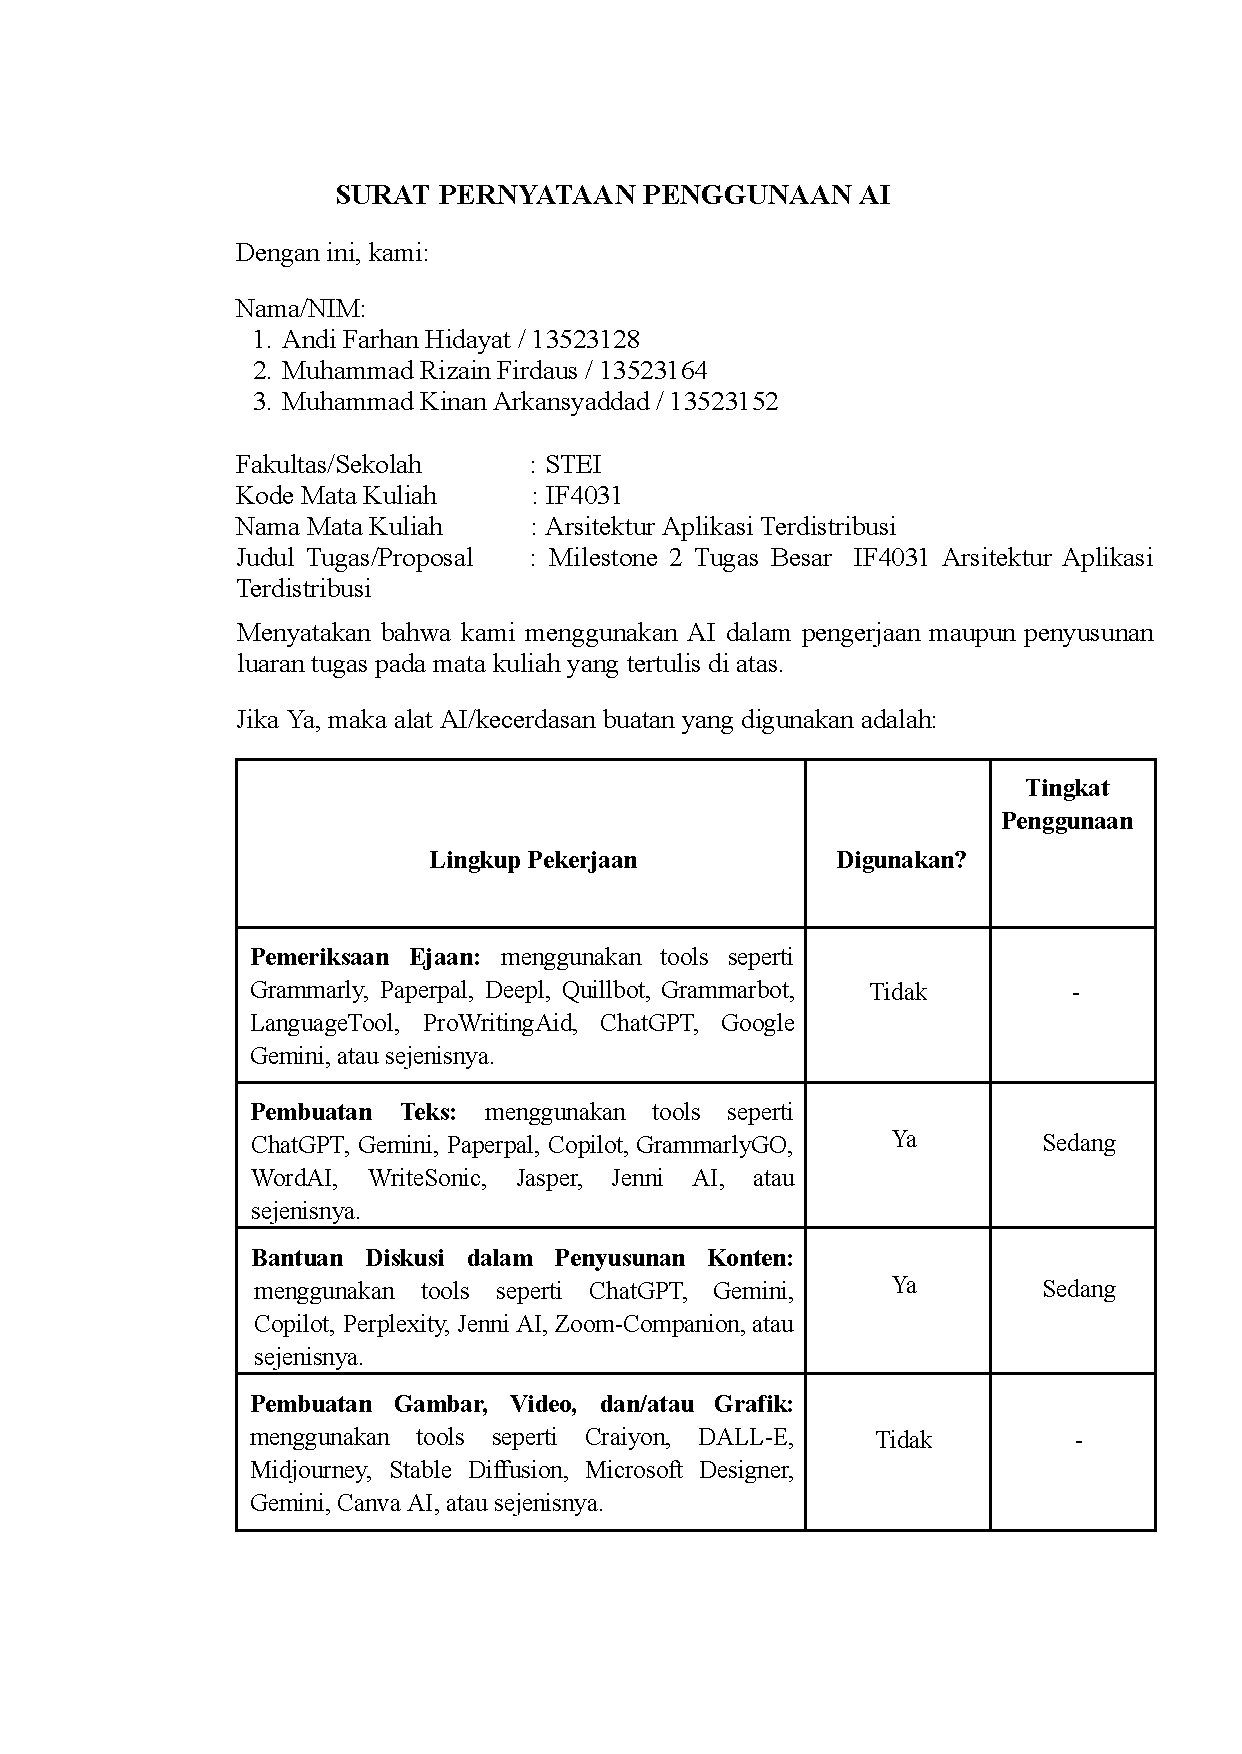
\includepdf[pages=-,pagecommand={\thispagestyle{empty}}]{signed.pdf}
\end{document}
